\chapter{Technical Coordination}
\label{ch:fdsp-coord}

Technical Coordination (TC) is responsible for detector integration
and installation support. 
%The technology for massive noble liquid detectors has developed over the last \num{45} years and the first large \dword{lartpc} was completed in 2010. While multiple \dwords{lartpc} have operated worldwide, the technology is still relatively new and the scale up to \dword{dune} presents challenges. However, the technology is well suited to massive neutrino detectors with millimeter scale resolution on \SI{100}{m} scale detectors and the technical challenges are surmountable.
The \dword{dune} collaboration consists of a large number of
institutions distributed throughout the world. They are supported by a
large number of funding sources and collaborate with a large number of
commercial partners. Groups of institutes within \dword{dune} form
consortia that take complete responsibility for construction of their
system.  \dword{dune} has empowered several consortia (currently nine)
with the responsibility to secure funding and design, fabricate,
assemble, install, commission and operate their components of the
\dword{dune} far detector. There are three consortia focussing
exclusively on the single phase detector: anode plane assembly (APA),
cold electronics (SPCE) and photon detector (SPPD). There are three
focussing exclusively on the dual phase detector: charge readout
plance (CRP), cold electronics (DPCE) and photon detector
(DPPD). There are three joint consortia: high voltage (HV), data
acquisition (DAQ) and cryogenic instrumentation and slow control
(CISC).  \dword{dune} Technical Coordination, under the direction of
the \dword{dune} Technical Coordinator, has the responsibility to
monitor the technical aspects of the detector construction, to
integrate and install the detector and to deliver the common projects. The
\dword{dune} TC organization is shown in Fig.~\ref{fig:TC_orgchart}.
\begin{figure}[htb]
  \begin{center}
    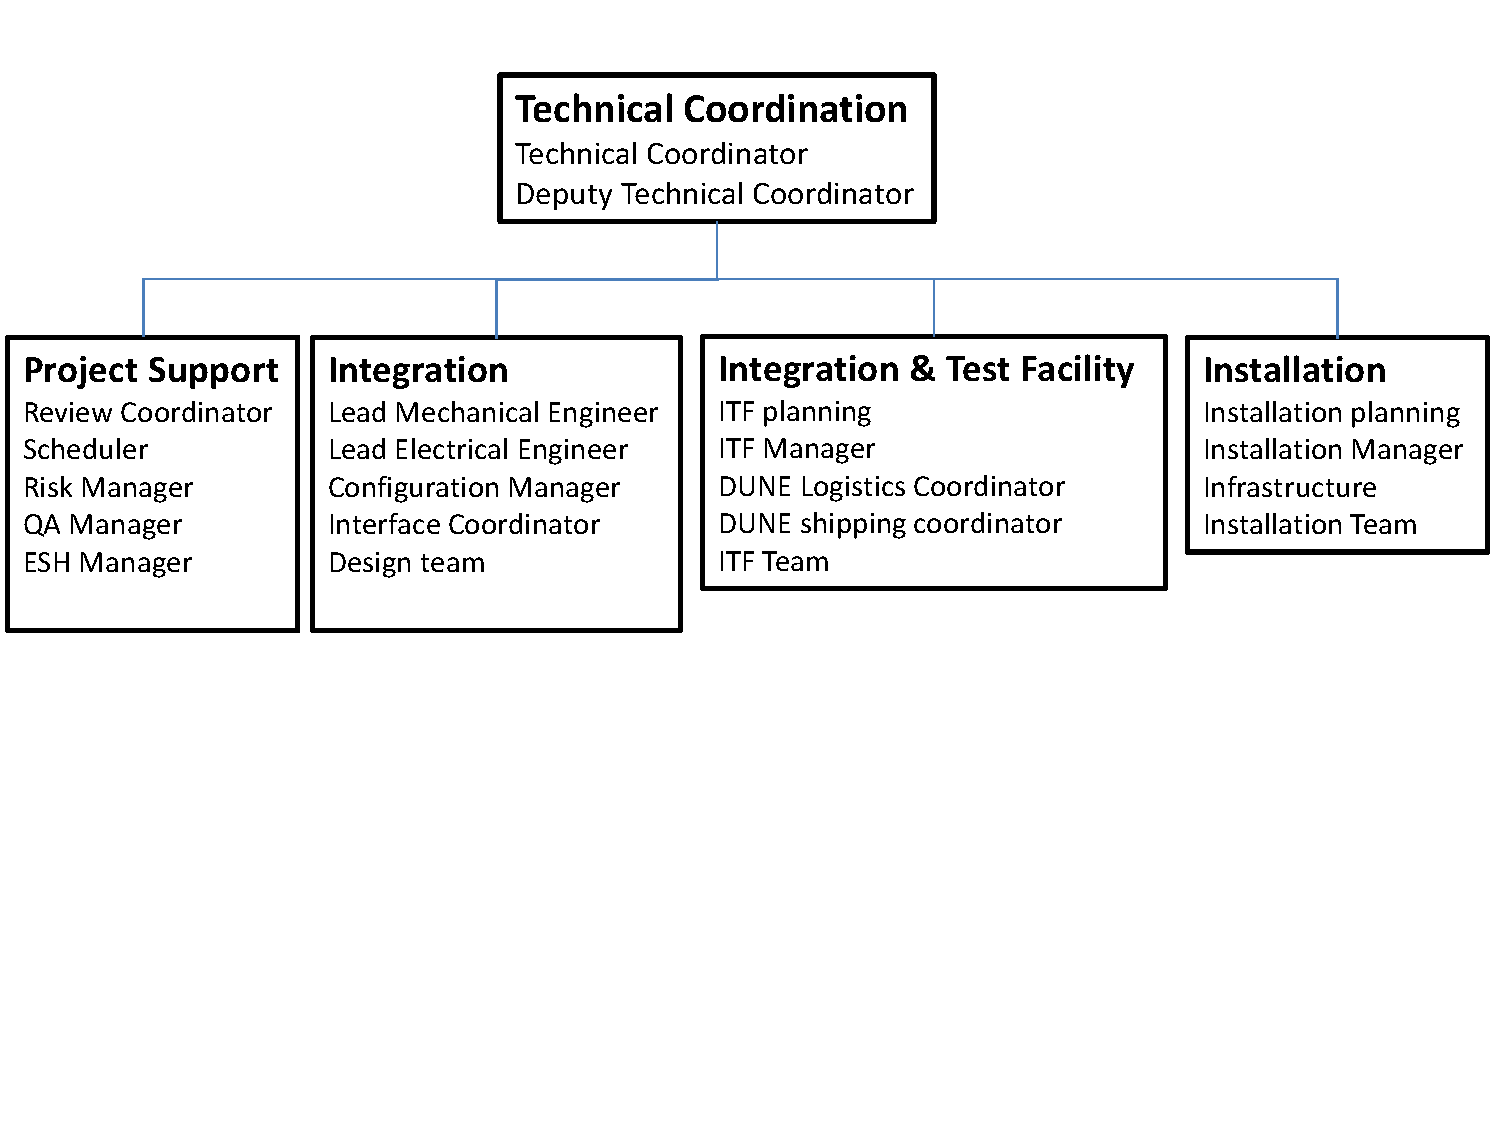
\includegraphics[width=0.8\textwidth]{far-detector-generic/figures/TP_TC_Org_Chart}
    \caption{Organization of Technical Coordination. This organization
      oversees the construction of the far detector, both single and
      dual phase, and the near detector.}
    \label{fig:TC_orgchart}
  \end{center}
\end{figure}
The TC organization staffing will grow over time as the project
advances. TC will provide staffing for teams underground at SURF, at
integration facilities and at the near site at FNAL.

The \dword{dune} Project consists of a \dword{fd} and a
\dword{nd}. The \dword{nd} is at a pre-conceptual state; as the
Conceptual Design and organization emerges, it will become part of the
\dword{dune} Project. Currently the \dword{dune} Project consists of
the \dword{dune} \dword{fd} consortia and Technical Coordination.  The
\dword{dune} Project is moving towards a Technical Design Report for
the far detector, both single and dual phase options, in 2019. It is
expected that a Conceptual Design Report for the \dword{nd} will be
prepared at the same time. Far detector components will be shipped
from the consortia construction sites to the the integrataion \& test
facility. TC will accept consortia components and oversee the
integration of components as appropriate. The scope of the
far detector intgegration and installation effort is shown graphically in
Fig.~\ref{fig:TC_flow}.
\begin{figure}[htb]
  \begin{center}
    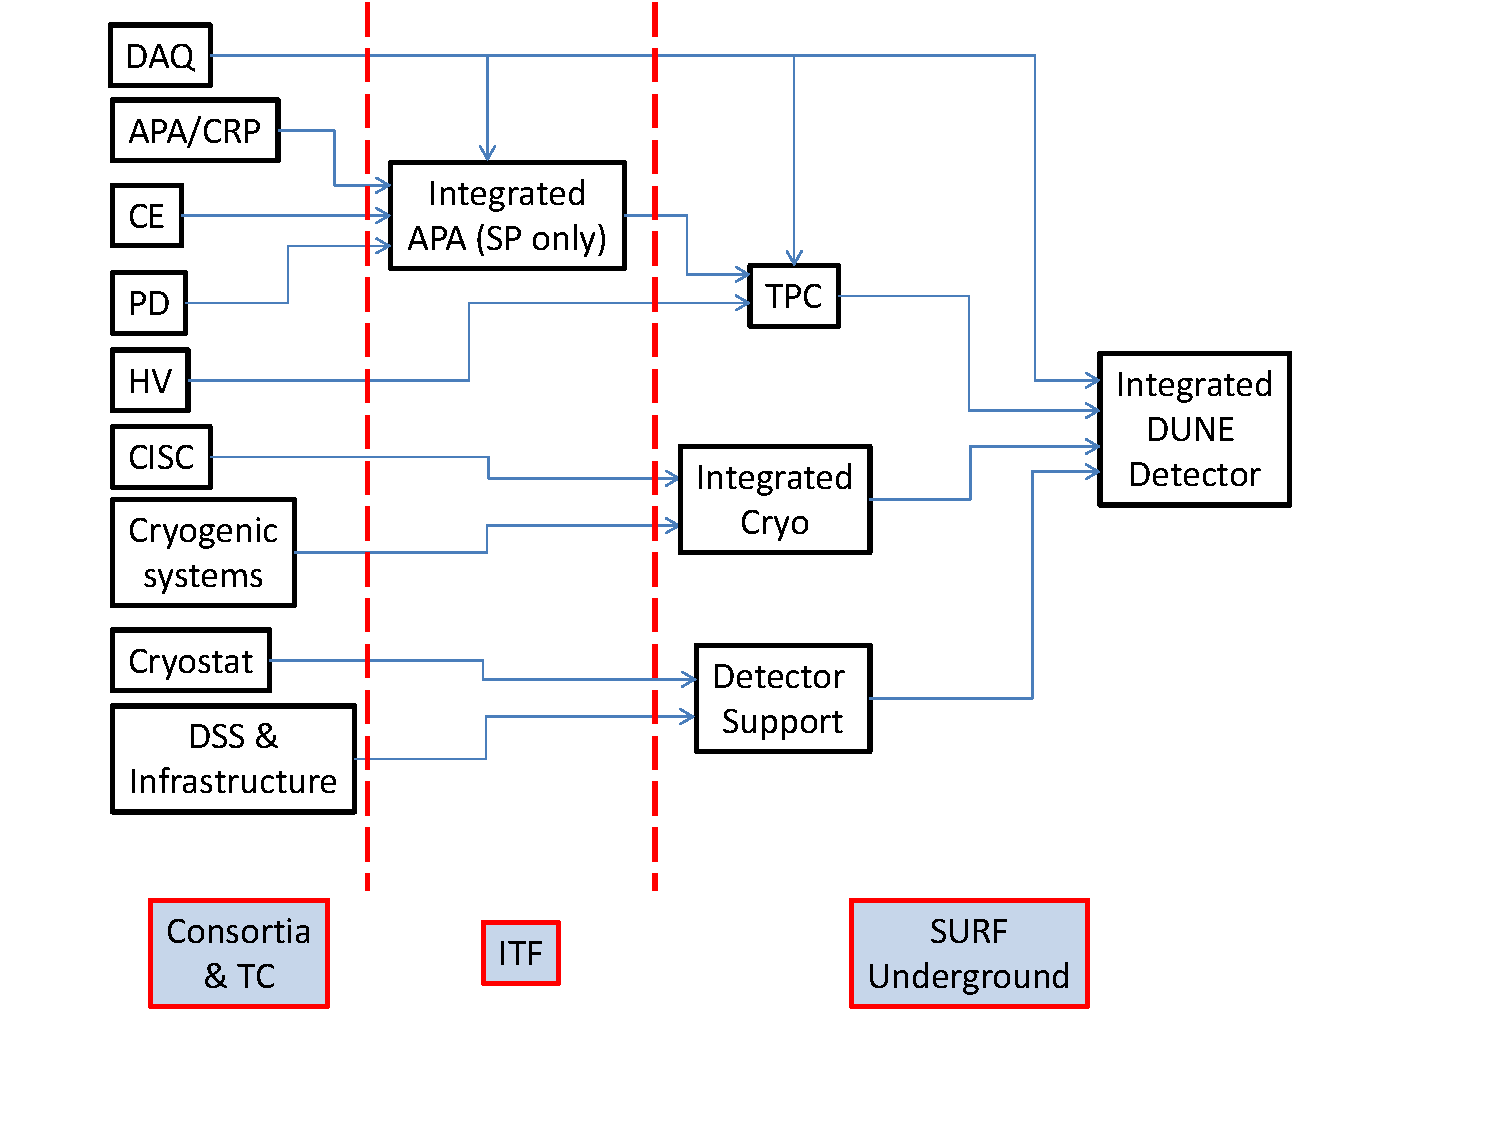
\includegraphics[width=0.8\textwidth]{far-detector-generic/figures/DUNE_deliverable_flow}
    \caption{Flow of components from the consortia to the far detector.}
    \label{fig:TC_flow}
  \end{center}
\end{figure}

TC interacts with the consortia via three main areas: project
coordination, integration and installation.  Construction of the
\dword{dune} Detector requires careful technical coordination due to
its complexity.  Given the horizontal nature of the consortia
structure and the extensive interdependencies between the systems, a
significant engineering organization is required to deliver
\dword{dune} on schedule and within specifications and funding
constraints.

The responsibilities of Technical Coordination include:
\begin{itemize}
  \item management and delivery of all common projects
  \item configuration control of all interface drawings and envelopes
  \item installation of detectors at the near and far sites
  \item logistics for detector integration and installation at the near and far sites
  \item survey of the detector
  \item primary interface to \dword{lbnf} for conventional facilities, cryostat and cryogenics
  \item primary interface to the Host Lab for infrastructure and operations support (\dword{lbnf}?)
  \item development and tracking of project schedule and milestones
  \item review of all aspects of the project
  \item recording and approving all project engineering information, including: documents, drawings and models
  \item project work breakdown schedules
  \item project risk register
  \item \dword{dune} engineering and safety standards, including grounding \& shielding
  \item monitoring of all consortia design and construction progress
  \item quality assurance and all QA related studies and documents
  \item ES\&H organization and all saftey related studies and documents
\end {itemize}

\dword{dune} TC interacts with \dword{lbnf} though the
\dword{lbnf}/\dword{dune} systems engineering organization. TC
provides the points of contact between the consortia and \dword{lbnf}.
TC will work with the \dword{lbnf}/\dword{dune} Systems Engineer to
implement the \dword{lbnf}/\dword{dune} Configuration Management Plan
to assure that all aspects of the overall \dword{lbnf}/\dword{dune}
project are well integrated. TC will work with \dword{lbnf} and the
Host Lab to ensure that adequate infrastructure and operations support
are provided during construction, integration, installation,
commissioning and operation of the detectors. The LBNF/DUNE systems
engineering organization is shown in Fig.~\ref{fig:DUNE_SE_org}.
\begin{figure}[htb]
  \begin{center}
    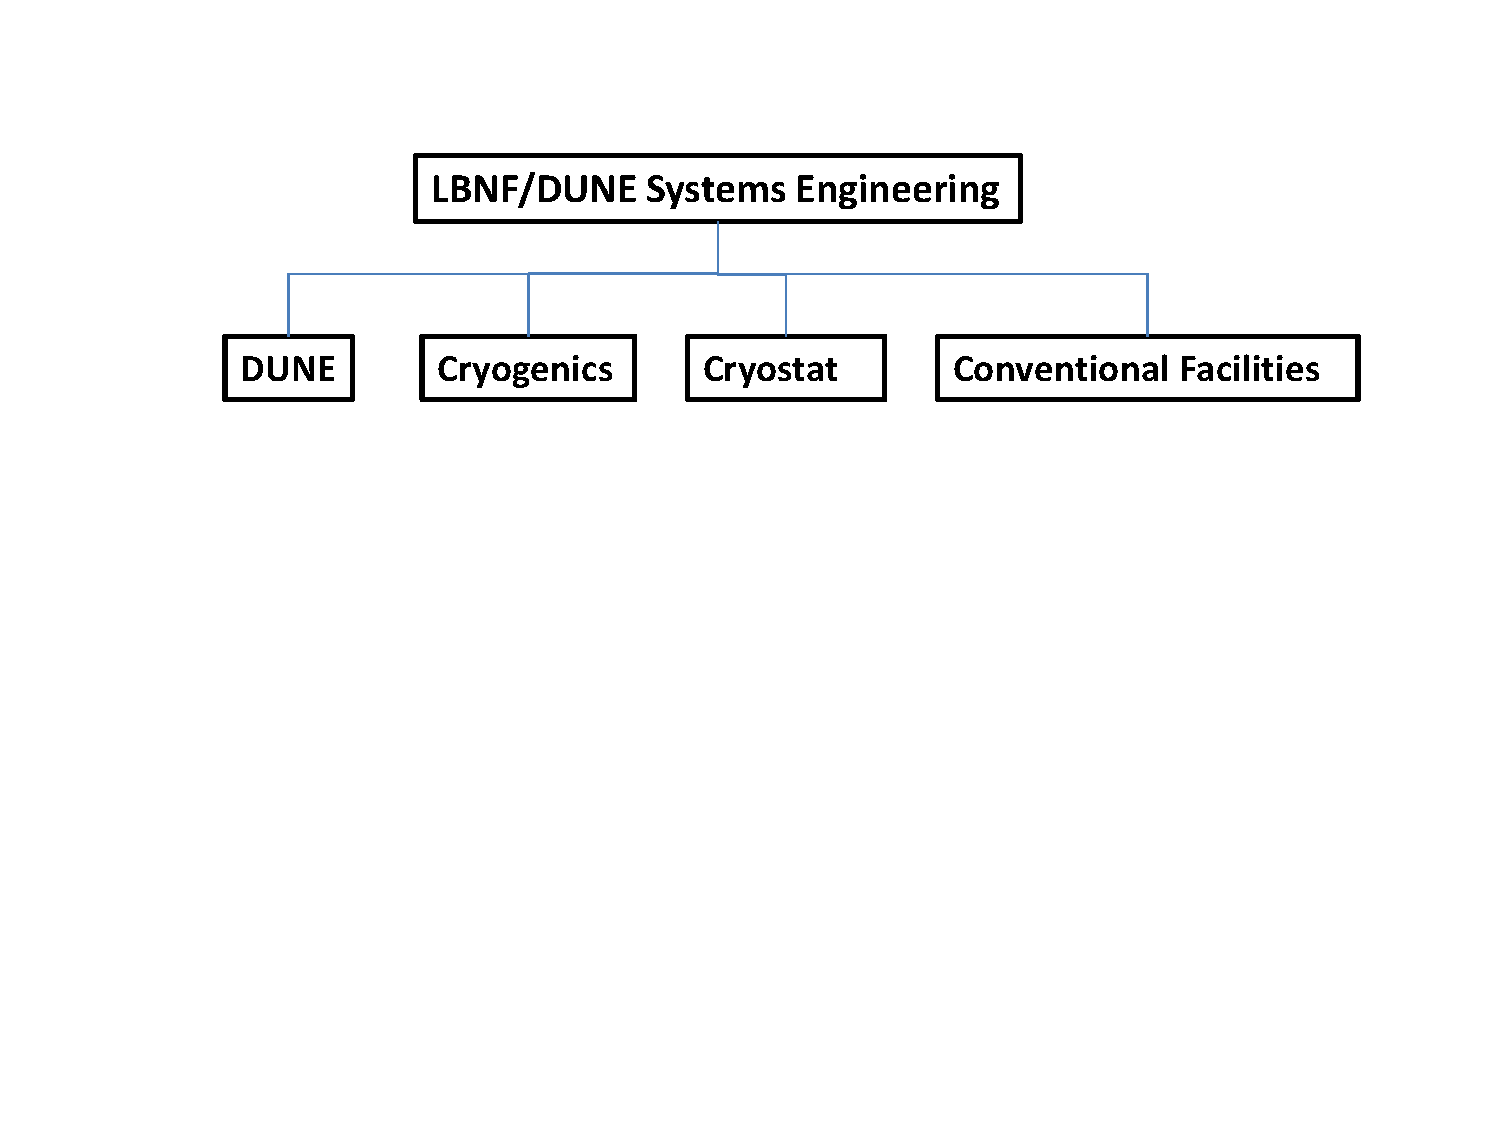
\includegraphics[width=0.8\textwidth]{far-detector-generic/figures/TC_SE_Org_Chart}
    \caption{LBNF/DUNE systems engineering organizational structure.}
    \label{fig:DUNE_SE_org}
  \end{center}
\end{figure}
TC has been working with the LBNF/DUNE systems engineering team to
define requirements from DUNE for the conventional facilities final
design. TC is representing the interests of the DUNE detector in the
CF design. This includes refining the detector installation plan to
understand how much space is needed in front of the temporary
construction openings (TCO) of the cryostats and therefore of the size
of the chambers. TC continues to refine the detector needs for
utilities in the detector caverns and the central utility cavern where
the DAQ will be housed.

Physics requirements on TC include cleanliness in the cryostats,
survey and alignment tolerances and grounding \& shielding
requirements. The cleanliness requirement is for ISO 8 (class
100,000), which will keep rates from dust radioactivity below those of
the inherent $^{39}$Ar background. The alignment tolerances are driven
by physics requirements on reconstructing tracks. Grounding and
shielding is critical to enable this very sensitive, low noise
detector to achieve the required signal to noise.

\section{Project Support}
\label{sec:fdsp-coord-supp}

The \dword{dune} Project is coordinated by Technical Coordination
(TC). The \dword{dune} Project consists of a \dword{fd} and a
\dword{nd}. The \dword{nd} is at a pre-conceptual state; as the
Conceptual Design and organization emerges, it will become part of the
\dword{dune} Project. Currently the \dword{dune} Project consists of
the \dword{dune} \dword{fd} consortia and Technical Coordination.  The
\dword{dune} Project is moving towards a Technical Design Report for
the far detector, both single and dual phase options, in 2019. It is
expected that a Conceptual Design Report for the \dword{nd} will be
prepared at the same time. A high level version of the \dword{dune}
Project schedule can be seen in Fig.~\ref{fig:DUNE_schedule}.
\begin{figure}[htb]
  \begin{center}
    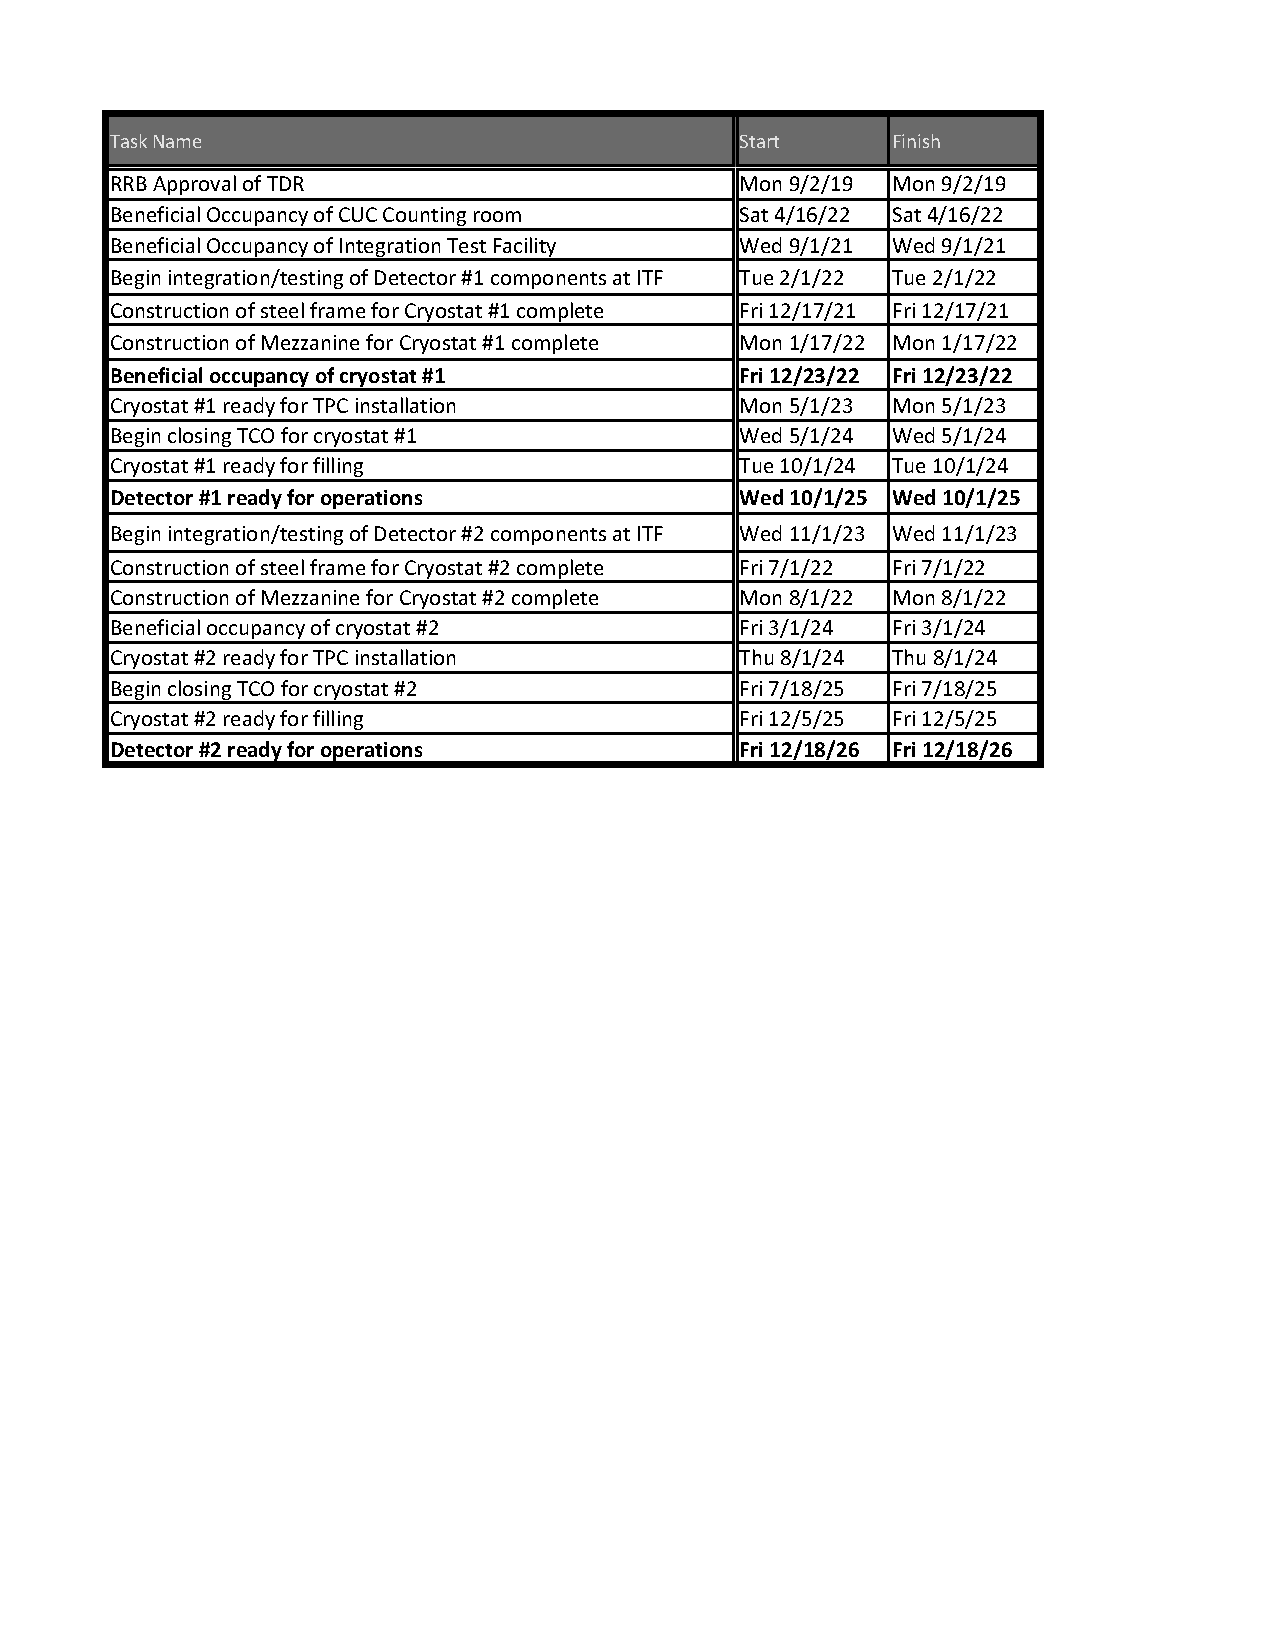
\includegraphics[width=0.8\textwidth]{far-detector-generic/figures/FD_Cnst_Schedule}
    \caption{Overall DUNE Project schedule.}
    \label{fig:DUNE_schedule}
  \end{center}
\end{figure}


As defined in the \dword{dune} Management Plan (DMP), the \dword{dune}
Technical Board (TB) is the technical decision making body for the
collaboration. It consists of all consortia scientific and technical
leads. It reports through the Executive Board (EB) to Collaboration
Management. The \dword{dune} Technical Board is chaired by the
Technical Coordinator. The DUNE collaboration management is shown in
Fig.~\ref{fig:DUNE_org}.
\begin{figure}[htb]
  \begin{center}
    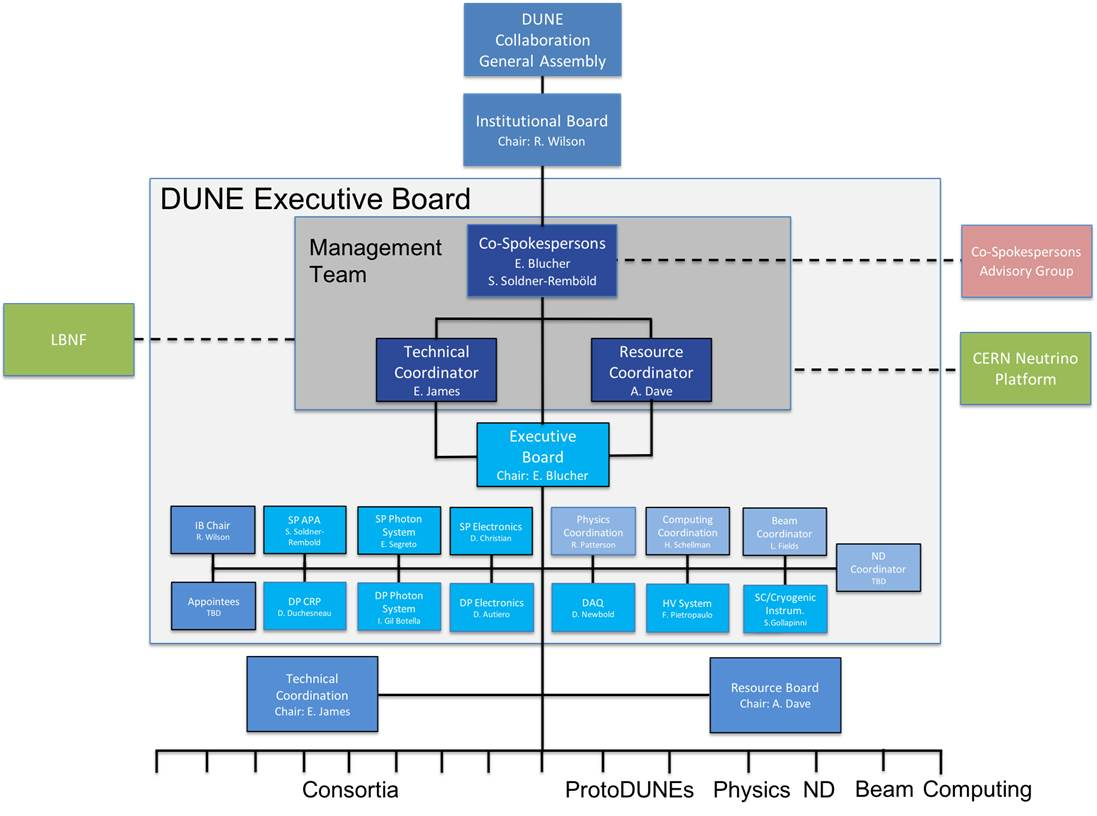
\includegraphics[width=0.8\textwidth]{far-detector-generic/figures/DUNE_mgmt}
    \caption{DUNE management organizational structure.}
    \label{fig:DUNE_org}
  \end{center}
\end{figure}



TC will work with the \dword{lbnf}/\dword{dune} Systems Engineer to
implement the \dword{lbnf}/\dword{dune} Configutation Management Plan
to assure that all aspects of the overall \dword{lbnf}/\dword{dune}
project are well integrated. TC will work with \dword{lbnf} and the
Host Lab to ensure that adequate infrastructure and operations support
are provided during construction, integration, installation,
commissioning and operation of the detectors. The LBNF/DUNE systems
engineering organization is shown in Fig.~\ref{fig:DUNE_SE_org}.
\begin{figure}[htb]
  \begin{center}
    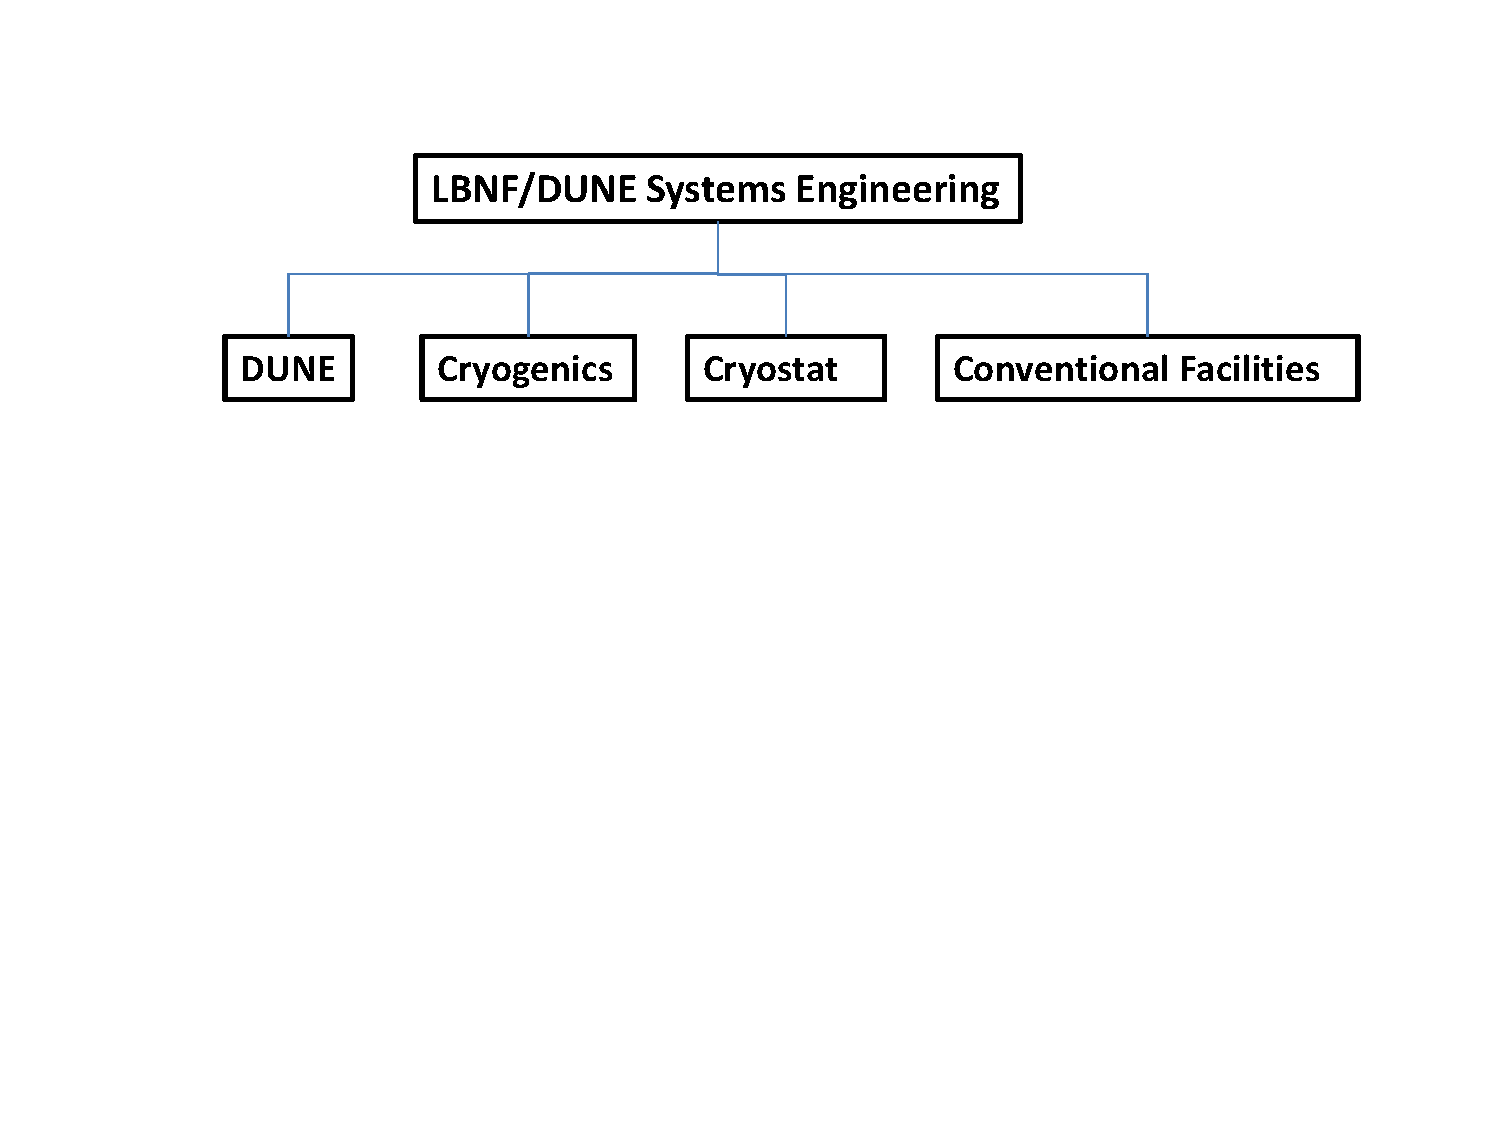
\includegraphics[width=0.8\textwidth]{far-detector-generic/figures/TC_SE_Org_Chart}
    \caption{LBNF/DUNE systems engineering organizational structure.}
    \label{fig:DUNE_SE_org}
  \end{center}
\end{figure}



Several major project support tasks need to be accomplished in advance
of the TDR:
\begin{itemize}
  \item Assure that each consortia has a well defined
and complete scope, that the interfaces between the consortia are
sufficiently well defined and that any remaining scope can be covered
by TC through Common Fund.
  \item Develop an overall project schedule that includes reasonable
production schedules from each consortia, well developed QA and QC
plans and a well developed installation schedule.
  \item Ensure that appropriate engineering and safety standards are
developed and agreed to by all key stakeholders and that these
standards are conveyed to and understood by each Consortium.
  \item Ensure that all \dword{dune} requirements on \dword{lbnf} for
conventional facilities, cryostat and cryogenics have been clearly
defined and understood by each Consortia.
  \item Ensure that all technical issues associated with scaling from
\dword{protodune} have sufficient resources to converge on decisions that
enable the detector to be fully integrated and installed.
  \item Ensure that the integration and QC processes for each
consortia are fully developed and reviewed and that the requiements on
an Integration and Test Facility are well defined.
\end{itemize}

%%%%%%%%%%%%%%%%%%%%%%%%%%%%%%%%
\subsection{Project Schedule}
\label{sec:fdsp-coord-controls}

Technical Coordination Project Controls (TCPC) maintains a web page
(currently located at
\href{https://web.fnal.gov/collaboration/DUNE/DUNE\%20Project/\_layouts/15/start.aspx\#/})
with links to project documents. TC maintains repositories of project
documents and drawings. These include the WBS, Schedule, risk
register, requirements, milestones, strategy, detector models and
drawings that define the \dword{dune} detector.

DUNE Project documents will be stored in DocDB. DUNE drawings will be stored in EDMS.

In order to ensure that the \dword{dune} detector remains on schedule, TCPC
will monitor schedule statusing from each consortium, will organize
reviews of schedules and risks as appropriate. TCPC will maintain a
master schedule that links all consortia schedules and contains
appropriate milestones to monitor progress. The master schedule will
go under change control after the TDR is approved.

The consortia have provided preliminary versions of risk analyses that
have been collected on the TCPC webpage. These will be developed into
an overall risk register that will be monitored and maintained by TCPC
in coordination with the consortia.

A schedule of key consortia activity in the period 2018--19 leading up
to the TDR has been developed.

A monthly report with input from all consortia will be published by
TCPC. This will include updates on consortia technical progress and
updates from TC.

Consortia have developed initial interface documents that will be put
under change control and managed by the TC integration engineering
team along with the consortia involved. These are currently in DocDB
and will likely go under change control later in 2018, although they
will continue to be developed through the TDR.

TCPC will maintain approved versions of QA, QC and testing plans,
installation plans, engineering and safety standards,...

A series of tiered milestones are being developed for the \dword{dune}
project. The Tier-0 milestones are held by the Spokespersons and Host
Lab director. Three have been defined and the current target dates
are:
\begin{enumerate}
\item Start main cavern excavation \hspace{2.1in} 2019
\item Start detector \#1 installation \hspace{2.1in} 2022
\item Start operations of detector \#1--2 with beam \hspace{1in} 2026
\end{enumerate}
These dates will be revisited at the time of the TDR review.  Tier-1
milestones will be held by the Technical Coordinator and \dword{lbnf} Project
Manager and will be defined in advance of the TDR review. Tier-2
milestones will be held by the Consortia.


%%%%%%%%%%%%%%%%%%%%%%%%%%%%%%%%
\subsection{Risk}
\label{sec:fdsp-coord-risk}

The successful operation of \dword{protodune} will retire a great many
potential risks to \dword{dune}. This includes most risks associated with the
technical design, production processes, quality assurance, integration
and installation. Residual risks remain relating to design and
production modifications associated with scaling to \dword{dune}, mitigations
to known installation and performance issues in \dword{protodune}, underground
installation at SURF and organizational growth.

[Enumerate remaining technical risks?.... or all risks?.... 600kV, HV
  in general, noise, dead channels, 20 year operation, QC in general,
  ADC/coldata, photon light yield, purity, LAr surface stbility, LEM
  gain, dual-phase LAr surface cleanliness, cathode/FC discharge to
  cryostat, incomplete calibration plan, incomplete connection of
  design to physics; funding, production schedule, integration plan,
  testing, underground installation, ...]

Key risks for TC to manage include the following:
\begin{enumerate}
  \item A key risk for TC is to ensure that sufficient scope is funded
    by the Consortia, such that the deliverables from TC do not grow
    so large as to be unsupportable by Common Fund.
  \item The second key risk is to ensure that key stakeholders to this
    first international mega-science project hosted in the US,
    including TC, FNAL as Host Lab, SURF, DOE and all international
    partners continue to successfully work together to ensure
    appropriate rules and services are provided to enable success of
    the project.
  \item The third key risk is to ensure that TC obtains sufficient
    personnel resources so as to be able to ensure that TC can oversee
    and coordinate all of its project tasks.  While the US has a
    special responsibility towards TC as host country, it is expected
    that personnel resources will be directed to TC from each
    collaborating country. Related to this risk is the fact that
    consortia deliverables are not really stand-alone subsystems; they
    are all parts of a single TPC. This elevates the requirements on
    coordination between consortia.
\end{enumerate}



%%%%%%%%%%%%%%%%%%%%%%%%%%%%%%%%
\subsection{Reviews}
\label{sec:fdsp-coord-reviews}

Technical Coordination is responsible to review all stages of detector
development and works with each consortium to arrange reviews of the
design, production readiness, production progress and operational
readiness of their system.  These reviews provide input for the TB to
make technical decisions.  Review reports are tracked by TC and
provide guidance as to key issues that will require engineering
oversight by the TC integration engineering team. TCPC will maintain a
calendar of \dword{dune} reviews.

TC will work with consortia leaders to review all detector designs,
with an expectation for a preliminary design review, followed by a
final design review. All major technology decisions will be reviewed
prior to down-select.

Start of production of all DUNE detector elements can commence after
successful production readiness review. Consortia should expect
regular production progress reviews once production has commenced.

%%%%%%%%%%%%%%%%%%%%%%%%%%%%%%%%
\subsection{Quality Assurance}
\label{sec:fdsp-coord-qa}


The \dword{lbnf}/\dword{dune} Quality Assurance Plan outlines the QA
requirements for all \dword{dune} Consortia and describes how the
requirements shall be met. The Consortia will be responsible for
implementing a quality plan that meet the requirements of the
\dword{lbnf}/\dword{dune} Quality Assurance Plan.  The Consortia
implement the plan through the development of individual quality
plans, procedures, guides, QC inspection and test requirements and
travelers/test reports.  In lieu of a Consortia Specific Quality Plan,
the Consortia may work under the \dword{lbnf}/\dword{dune} Quality
Assurance Plan and develop Manufacturing/QC Plans, procedures and
documentation specific to their work scope.  The \dword{dune}
Technical Coordinator and Consortia Leaders are responsible for
providing the resources needed to conduct the Project successfully,
including those required to manage, perform and verify work that
affects quality.  The \dword{dune} Consortia Leaders are responsible
for identifying adequate resources to complete the work scope and to
ensure that their team members are adequately trained and qualified to
perform their assigned work.

The Consortia work will be documented on travelers and applicable test
or inspection reports. Records of the fabrication, inspection and
testing will be maintained. When a component has been identified as
being in noncompliance to the design, the nonconforming condition
shall be documented, evaluated and dispositioned as use-as-is (does
not meet design but can meet functionality as is), rework (bring into
compliance with design), repair (will be brought into meeting
functionality but will not meet design) and scrap.

The \dword{lbnf}/\dword{dune} Quality Assurance Manager (QAM) reports
to the \dword{lbnf} Project Manager and \dword{dune} Technical
Coordinator and provides oversight and support to the Consortia
Leaders to ensure a consistent quality program.
\begin{enumerate}
  \item The QAM will plan reviews as independent assessments to assist
    the \dword{dune} Technical Coordinator in identifying opportunities for
    quality/performance-based improvement and to ensure compliance
    with specified requirements.
  \item The QAM is responsible to work with the Consortia in
    developing their QA/QC Plans.
  \item The QAM will review Consortia QA/QC activity, including
    production site visits.
  \item The QAM will participate in Consortia Design Reviews, conduct
    Production Readiness Reviews prior to the start of production,
    conduct Production Progress Reviews on a regular basis, and
    perform follow-up visits to Consortia facilities prior to shipment
    of components to ensure all components and documentation are
    satisfactory.
\item The QAM is responsible for performing assessments at the
  Integration Facility, the Far Site and the Near Site to
  ensure the activities performed at these locations are in accordance
  with the \dword{lbnf}/\dword{dune} QA Program and applicable procedures,
  specifications and drawings.
\end{enumerate}

%%%%%%%%%%%%%%%%%%%%%%%%%%%%%%%%
\subsection{ES\&H}
\label{sec:fdsp-coord-esh}

The \dword{dune} Environmental, Safety and Health (ESH) program is described
in the \dword{lbnf}/\dword{dune} Integrated Environmental, Safety and Health
Plan. This plan is maintained by the \dword{lbnf}/\dword{dune} ESH Manager, who
reports to the \dword{lbnf} Project Manager and the TC. The ESH is responsible
to work with the Consortia in reviewing their hazards and their ESH
plans.  The ESH Manager is responsible to review ESH at production
sites, integration sites and at SURF.

\section{Integration}
\label{sec:fdsp-coord-integ-sysengr}
%				7 pages

The major aspects of detector integration focus on the mechanical and
electrical connections between each of the detector systems. A second
major area is in the support of the detector and its interfaces to the
cryostat. A third major area is in assuring that the detector can be
installed --- that the integrated components can be moved into their
final configuration. A fourth major area is in the integration of the
detector with the necessary services provided by the conventional
facilities.

%%%%%%%%%%%%%%%%%%%%%%%%%%%%%%%%
\subsection{Configuration Management}
\label{sec:fdsp-coord-integ-config}

The \dword{dune} Technical Coordination engineering team will maintain
full 3-D CAD models of the detectors, and the consortia will be
responsible for providing the team with CAD models of their detector
components for integration into the overall models.  The project
engineering team will work with the \dword{lbnf} project team to integrate the
full detector models into a global \dword{lbnf} CAD model that includes
cryostats, cryogenic systems, and the conventional facilities.  The
\dword{dune} project engineering team will work directly with the consortia
Technical Leads and their supporting engineering teams to resolve any
detector component interference and connection issues with other
detector systems, detector infrastructure, and facility
infrastructure.

For mechanical design aspects, the \dword{dune} TC 
engineering team will maintain full 3-D CAD models of the detectors.
Each consortium will be responsible for providing the project
engineering team with CAD models of their detector components to be
integrated into overall models.  The TC engineering team will
work with the \dword{lbnf} project team to integrate the full detector models
into a global \dword{lbnf} CAD model that will include cryostats, cryogenic
systems, and the conventional facilities.  The TC
engineering team will work directly with the consortia Technical Leads
and their supporting engineering teams to resolve any detector
component interference and/or connection issues with other detector
systems, detector infrastructure, and facility infrastructure.

For electrical design aspects, the TC
engineering team will maintain high level interface documents which
describe all aspects of required electrical infrastructure and
electrical connections.  All consortia must document power
requirements and rack space requirements.  Consortia are responsible
for defining any cabling which bridges the design efforts of two or
more consortia.  This agreed upon and signed-off interface
documentation should include cable specification, connector
specification, connector pinout and any data format, signal levels and
timing.  All cables, connectors, printed circuit board components,
physical layout and construction will be subject to project review.
This is especially true of elements which will be inaccessible during
the project lifetime.  Consortia should provide details on liquid
argon temperature acceptance testing and lifetime of components,
boards, cables and connectors.


At the time of the release of the Technical Design Reports, the
project engineering team will work with the consortia to produce
formal engineering drawings for all detector components.  These
drawings are expected to be signed by the consortia Technical Leads,
project engineers, and Technical Coordinator.  Starting from that
point, the detector models and drawings will sit under formal change
control.  It is anticipated that designs will undergo further
revisions prior to the start of detector construction, but any changes
made after the release of the Technical Design Reports will need to be
agreed to by all of the drawing signers and an updated, signed drawing
produced.

The major areas of configuration management include:
\begin{enumerate}
  \item 3-D Model
  \item Interface Definitions
  \item Envelope Drawings for installation
  \item Drawing management
\end{enumerate}

%%%%%%%%%%%%%%%%%%%%%%%%%%%%%%%%
\subsubsection{Configuration Management Processes}
\label{ssec:fdsp-coord-integ-cnfg-mgmt}

\fixme{redundant with 9.1.5.1}
Technical Coordination will put into place processes for
configuration management.  Configuration management will provide
technical coordination and engineering staff the ability to define and
control the actual build of the detector at any point in time and to
track any changes which may occur over duration of the build as well
as the lifetime of the project.

For detector elements within the cryostat, configuration management
will be frozen once the elements are permanently sealed within the
cryostat.  However, during the integration and installation process of
building the detector within the cryostat, changes may need to occur.
For detector elements outside the cryostat and accessible, all
repairs, replacements, hardware upgrades, system grounding changes,
firmware and software changes must be tracked.

Any change will require revision control, configuration
identification, change management and release management.

{\bf Revision Control}\\ Consortia will be responsible for providing
accurate and well documented revision control.  Revision control
should provide a method of tracking and maintaining the history of
changes to a detector element.  Each detector element must be clearly
identified with a document which includes a revision number and
revision history.  For mechanical elements, this will be reflected by
a drawing number with revision information.  For electrical elements,
schematics will be used to track revisions.  Consortia will be
responsible for identifying the revision status of each installed
detector elements. Revisios are further controlled through maintenance
of the documents in DocDB.

{\bf Configuration Identification}\\
Consortia are responsible for providing unique identifiers or part
numbers for each detector element.  Plans will be developed on how
inventories will be maintained and tracked during the build.  Plans
will clearly identify any dynamic configuration modes which may be
unique to a specific detector element.  For example, a printed circuit
board may have firmware which effects its performance.

{\bf Change Management}\\
Technical Coordination will provide guidelines
for formal change management.  During the beginning phase of the
project, drawings and interface documents are expected to be signed by
the consortia Technical Leads, project engineers, and Technical
Coordinator.  Once this initial design phase is complete, the detector
models, drawings, schematics and interface documents will be under
formal change control.  It is anticipated that designs will undergo
further revisions prior to the start of detector construction, but any
changes made after the release of the Technical Design Reports will
need to be agreed to by all drawing signers and an updated signed
drawing produced.

{\bf Release Management}\\
Release management focuses on the delivery of the more dynamic aspects
of the project such as firmware and software.  Consortia with
deliverables that have the ability to effect performance of the
detector by changing firmware or software must provide plans on how
these revisions will be tracked, tested and released.  The
modification of any software or firmware after the initial release,
must be formally controlled, agreed upon and tracked.


%%%%%%%%%%%%%%%%%%%%%%%%%%%%%%%%
\subsection{Engineering process and support}
\label{sec:fdsp-coord-integ-engr-proc}
 

The \dword{dune} Technical Coordination organization will work with the
consortia through its TC engineering team to ensure the proper
integration of all detector components.  The TC engineering team
will document requirements on engineering standards and documentation
that the consortia will need to adhere to in the design process for
the detector components under their responsibility.  Similarly, the
project QA and ES\&H managers will document quality control and safety
criteria that the consortia will be required to follow during the
construction, installation, and commissioning of their detector
components, as discussed in sections~\ref{sec:fdsp-coord-qa} and {sec:fdsp-coord-esh}.


Consortia interfaces with the conventional facilities, cryostats, and
cryogenics are managed through the \dword{dune} Technical Coordination
organization.  The TC engineering team will work with the
consortia to understand their interfaces to the facilities and then
communicate these globally to the \dword{lbnf} project team.  For conventional
facilities the types of interfaces to be considered are requirements
for bringing needed detector components down the shaft and through the
underground tunnels to the detector cavern, overall requirements for
power and cooling in the detector caverns, and the requirements on
cable connections from the underground area to the surface.
Interfaces to the cryostat include the number and sizes of the
penetrations on top of the cryostat, required mechanical structures
attaching to the cryostat walls for supporting cables and
instrumentation, and requirements on the global positioning of the
detector within the cryostat.  Cryogenic system interfaces include
requirements on the location of inlet/output ports, requirements on
the monitoring of the liquid argon both inside and outside the
cryostat, and grounding/shielding requirements on piping attached to
the cryostat.

\dword{lbnf} will be responsible for the design and construction of the
cryostats used to house the detectors.  The consortia are required to
provide input on the location and sizes of the needed penetrations at
the top of the cryostats.  The consortia also need to specify any
mechanical structures to be attached to the cryostat walls for
supporting cables or instrumentation.  The \dword{dune} project engineering
team will work with the \dword{lbnf} cryostat engineering team to understand
what attached fixturing is possible and iterate with the consortia as
necessary.  The consortia will also work with the project engineering
team through the development of the 3-D CAD model to understand the
overall position of the detector within the cryostat and any issues
associated with the resulting locations of their detector components.

\dword{lbnf} will be responsible for the cryogenics systems used to purge,
cool, and fill the cryostats.  It will also be responsible for the
system that continually re-circulates liquid argon through filtering
systems to remove impurities.  Any detector requirements on the flow
of liquid within the cryostat should be developed by the consortia and
transmitted to \dword{lbnf} through the project engineering team.  Similarly,
any requirements on the rate of cool-down or maximum temperature
differential across the cryostat during the cool-down process should
be specified by the consortia and transmitted to the \dword{lbnf} team.



%%%%%%%%%%%%%%%%%%%%%%%%%%%%%%%%
\subsubsection{Engineering Processes}
\label{ssec:fdsp-coord-integ-eng-processes}

\fixme{redundant with 9.1.5.2}
The engineering design process is defined by a set of steps taken to
fulfill the requirements of the design.  By the time of the Technical
Design Report, all design requirements must be fully defined and
proposed designs must be shown meet these requirements.  Based on
prior work, some detector elements may be quite advanced in the
engineering process, while others may be in earlier stages.  Each
design process shall closely follow the engineering steps described
below.


{\bf Development of specifications}\\
Each consortium is responsible for the technical review and approval
of the engineering specifications.  The documented specifications for
all major design elements should include the scope of work, project
milestones, relevant codes and standards to be followed, acceptance
criteria and specify appropriate internal or external design reviews.
Specifications shall be treated as controlled documents and cannot be
altered without approval of the \dword{dune} Technical Coordination team.  The
TC engineering team will participate in and help facilitate all
major reviews.  Special Technical Board reviews will be scheduled for
major detector elements.

{\bf Engineering Risk Analysis}\\
Each consortium is responsible for identifying and defining the level
of risk associated with their deliverables.  \dword{dune} Technical
Coordination will work with the consortia, through its
TC engineering team, to document these risks in a Risk Database
and follow them throughout the project until they are realized or can
be retired.

{\bf Specification Review}\\
The \dword{dune} Technical Coordination organization and project engineers
shall review consortia specifications for overall compliance with the
project requirements.  Consortia must document all internal reviews
and provide that documentation to the Technical Coordination staff.
Additional higher level reviews may be scheduled by the Technical
Coordination staff.

{\bf System Design}\\
The system design process includes the production of mechanical
drawings, electrical schematics, calculations which verify compliance
to engineering standards, firmware, printed circuit board layout,
cabling and connector specification, software plans, and any other
aspects that lead to a fully documented functional design.  All
relevant documentation shall be recorded, with appropriate document
number, into the chosen engineering data management system and be
available for the review process.

{\bf Engineering Design Review}\\
The design review process is determined by the complexity and risk
associated with the design element.  For a simple design element, the
consortia may do an internal review.  For a more complex or high risk
element a formal review will be scheduled.  The \dword{dune} Technical
Coordination staff will facilitate the review, bringing in outside
experts as needed.  In all cases, the result of any reviews should be
well documented and captured in the engineering data management
system.  If recommendations are made, those recommendations will be
tracked in a database and the consortia will be expected to provide a
response.

{\bf Procurement}\\ The procurement process will include the
documented technical specifications for all procured materials and
parts.  All procurement technical documents are reviewed for
compliance to engineering standards, safety and environmental
concerns.  The \dword{dune} Technical Coordination staff will assist the
consortia in working with their procurement staff as needed.

{\bf Implementation}\\ During the implementation phase of the project,
the consortia shall provide the Technical Coordinator with updates on
schedule.  A test plan will fully developed which will allow for
verification that the initial requirements have been met. In addition,
a quality assurance plan will be documented and followed.

{\bf Testing and Validation\\}
The testing plan documented in the above step will be followed and
results will be well documented.  The Technical Coordinator and
engineering team will be informed as to the results and whether the
design meets the specifications.  If not, a plan will be formulated
to address any shortcomings and presented to the Technical
Coordinator. [QA Manager should be mentioned here]

{\bf Final Documentation\\}
Final reports should be generated which describes the as built
equipment, any lessons learned, safety reports, installation procedures
and checks, and operations manual.

\section{Installation Coordination and Support}
\label{sec:fdsp-coord-install}
%						15 pages

%%%%%%%%%%%%%%%%%%%%%%%%%%%%%%%%
%\subsection{Organization}
%\label{sec:fdsp-coord-org}

Installation Coordination and Support (or simply Installation) is
responsible for coordinating the detector installations, providing
detector installation support and providing installation related
infrastructure. The installation group management responsibility is
shared by a scientific lead and a technical lead that report to the
Technical Coordinator. The underground group will be referred to as
the \dword{uit}. The \dword{itf} group which delivers equipment to the
Ross Shaft and the \dword{uit} which receives the equipment
underground need to be in close communication and work closely
together.

Underground installation is in general responsible for coordinating
and supporting the installation of the detectors and providing
necessary infrastructure for installation of the experiment. While the individual
consortia are responsible for the installation of their own detector
equipment it is essential that the detector installation be planned
as a whole and that a single group coordinates the installation and
adapts the plans throughout the installation process. The \dword{uit} has 
responsibility for overall coordination of the installations. In
conjunction with each consortium the \dword{uit} will make the installation
plan that describes how the detectors are to be installed. The
installation plan is used to define the spaces and infrastructure that
will be needed to install the detectors. The installation plan will
also be used to define the interfaces between the Installation group
and the consortia deliverables.  The installation scope includes the
infrastructure needed to install the detector such as the cleanroom, a
small machine shop, special cranes, scissor lifts, and access equipment.
Additional equipment required for installation includes: rigging equipment, hand tools, diagnostic equipment
(including oscilloscopes, network analyzers and leak detector), local storage with some critical supplies and some PPE. The \dword{uit} will also provide trained personnel to operate the installation
infrastructure. The consortia will provide the detector elements and
custom tooling and fixtures as required to install their detector
components.
%In the case of the single-phase detector the installation
%group will also provide the detector support system (DSS) which
%supports the detector and is needed to bring equipment into the
%cryostat.

%In addition to the installation specific infrastructure the
%installation group will also be responsible for general detector
%infrastructure like electronics racks, cable trays, power, and if
%needed additional optical fibers in the shafts.

 

%The \dword{dune} production phases are divided into
%production setup and production. Scope that represents a one time
%investment is included in production setup while equipment and
%infrastructure that scales with the number of detectors is included in
%production. With this definition several of the possible work packages
%are empty. For example once the surface logistics facility is setup it
%will be used for all \num{4} detectors so its scope is completely under
%production setup.



%The organization of the full installation scope into
%work packages that are associated with the different phase of the
%project and the lower level WBS divisions are shown in
%Figure~\ref{WP_def}.
%\begin{figure}[!h]
 % \begin{center}
%   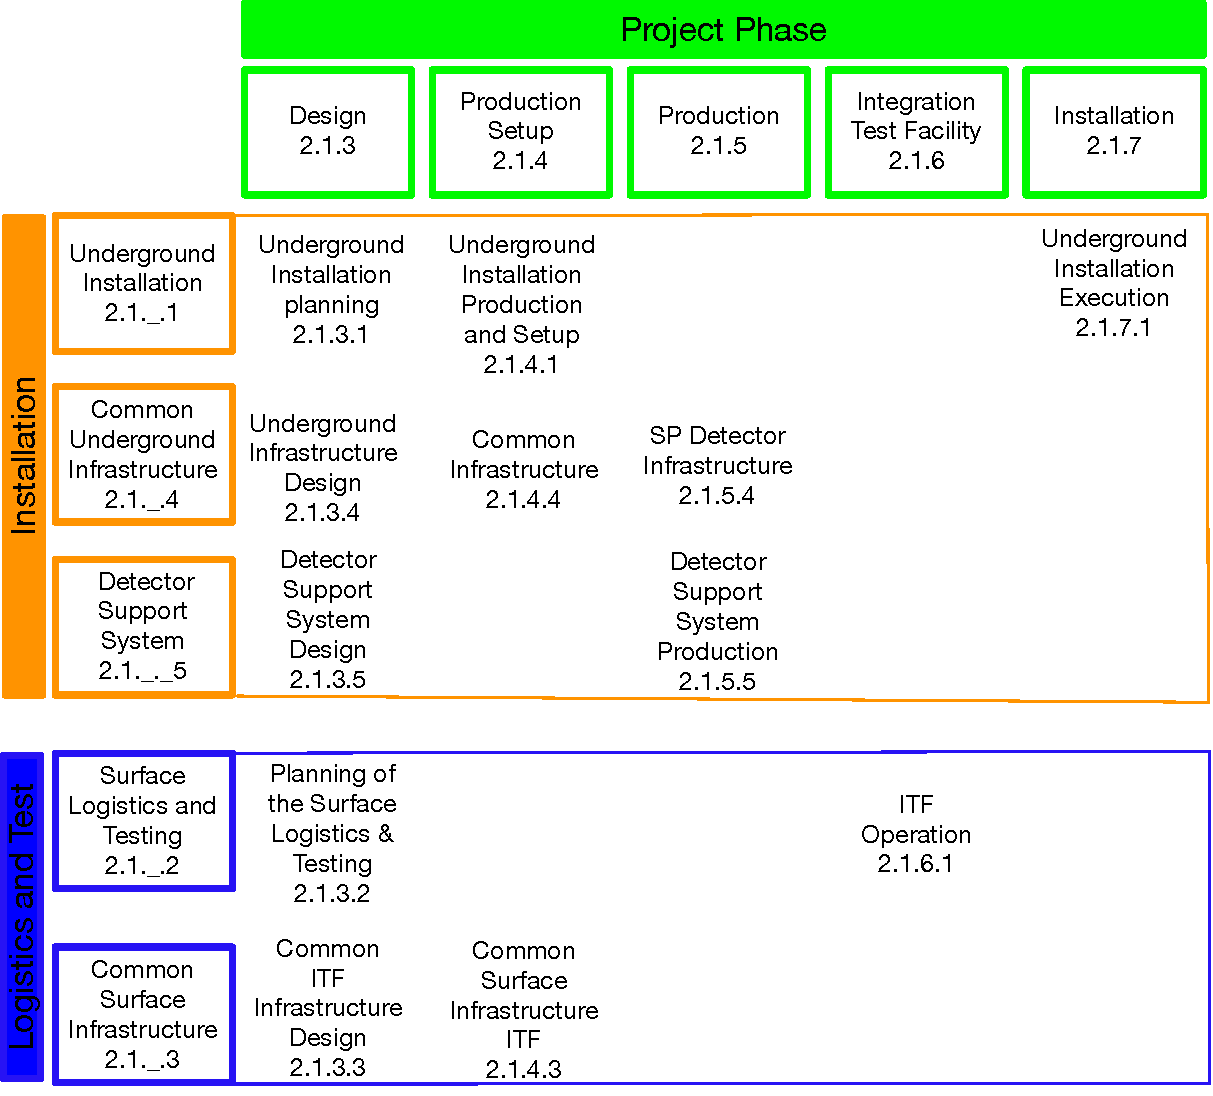
\includegraphics[width=0.8\textwidth]{far-detector-single-phase/figures/OrgChart-v3.pdf}
 %   \caption{Organization of installation and Surface Logistics and
%      Testing. The columns in the matrix represent the project phase
%      and the rows the major divisions in scope. Work packages define
%      the deliverables for each phase according to the major division
%      in scope. }
%    \label{WP_def}
%  \end{center}
%\end{figure}



%%%%%%%%%%%%%%%%%%%%%%%%%%%%%%%%%
\subsection{Surface Logistics \& Testing}
\label{sec:fdsp-coord-integ-test}

The logistics for integrating and installing the DUNE Far Detectors
and their associated infrastructure face a number of
challenges. Possible difficulties include the size and complexity of
the detector itself, the number of sites around the world that will be
fabricating detector and infrastructure components, the necessity for
protecting components from dust, vibration and shock during their
journey to the deep underground laboratory and the lack of space on
the surface near the Sanford Lab Ross Shaft. One mitigation
of these risks is the establishment of a DUNE
Integration and Test Facility (ITF) somewhere in the vicinity of
Sanford Lab. Such a facility and its associated staff would contribute
to DUNE in the following areas.
\begin{itemize}
  \item {\bf Transport Buffer:} Storage capacity for one month
    material in the vicinity of Sanford Lab. Handle packaging
    materials returned from underground laboratory.
  \item {\bf Re-packaging} Facilitate possible re-packaging of
    components before transport underground.
  \item {\bf Component Fabrication:} Possibly provide a capability for
    fabrication of components near Sanford Lab. Undergraduate science
    and engineering students from the South Dakota School of Mines and
    Technology (SDSM\&T) may contribute low cost effort to these
    fabrication activities.
  \item {\bf Component Integration:} Some integration activities may
    be best accomplished in proximity to Sanford Lab. A possible
    example is connecting photodetectors and cold electronics to APAs.
  \item {\bf Inspection, Testing and Repair:} Consortia will define
    their testing requirements including procedures and
    criteria. Consortia will also specify procedures in cases of test
    failure, for example, repair, return to source or discard.
  \item {\bf Visitor Support:} Consortia will likely send staff to the
    ITF for the integration, testing and installation of the consortia
    detector components. The ITF will provide temporary space,
    computer access, assistance personnel and other infrastructure
    support for DUNE visitors.
\item {\bf Outreach:} The ITF may be well located to support a public outreach program. The DUNE Experiment is likely to generate considerable public interest and addressing those interests is important to long-term public support for DUNE specifically and particle physics generally.
\end{itemize}

\subsubsection{Scope}
The scope of the ITF includes several possibly related but mostly
independent tasks. They are:
\begin{itemize}
\item{\bf Cryostat:} The scope of this item is the four cryostats
  planned for installation at the 4850 level of Sanford Lab. Cryostat
  components include the warm steel structure, the stainless steel membrane and
  the insulation. The logistics for the cryostat components will be
  managed by the cryostat installation contractor and LBNF logistics
  coordinator.  Most likely this function will be met with a
  commercial warehousing vendor, who will supply suitable space,
  loading and unloading facilities and a commercial inventory
  management and control system. The vendor will provide all required
  personnel effort as part of its contracted responsibilities.
\item{\bf Cryogenics Systems:} The cryogenics systems are also an LBNF
  responsibility and cryogenics system logistics will likely be
  managed by LBNF similarly to the logistics for the cryostat
  components.
%\item{\bf Cryostat Support Structure:} This structure is an LBNF responsibility and will likely be addressed similarly to the Cryostats and the Cryogenic Systems.
\item{\bf DUNE Detectors:} The DUNE Detectors are the responsibility
  of the Collaboration as implemented by the Consortia. The role of
  the ITF will vary for the several Consortia and a description of
  these various roles is a major topic of this document.
\end{itemize}

\subsubsection{Location }
A reasonable criterion for the location of the ITF is within about an
hour drive from Sanford Lab. That criterion yields the following
possibilities.
\begin{center}
\begin{tabular}{ |c|c| } \hline
{\bf Location} & {\bf 2016 Population}  \\ \hline 
Deadwood & 1,264  \\ 
Lead & 3,010  \\
Rapid City & 74,048  \\
Spearfish & 11,531  \\
Sturgis & 6,832  \\ \hline
\end{tabular}
\end{center}
Since infrastructure is correlated with population, Rapid City would seem the most likely
choice for location with Spearfish as a second possibility. In addition to overall infrastructure,
particular assets of Rapid City include proximity to SDSM\&T and a business community that is
possibly interested in incorporating a DUNE ITF into an overall regional development
program.
%Black Hills State University is located in Spearfish, but that institution is less technology oriented than SDSM\&T.

%$$$$$$$$$$
\subsubsection{\bf Requests from each consortia} 
In February of 2018, questionnaires were distributed to each consortia to seek
their requirements for ITF. Table~\ref{table:leders} lists leaders of each consortia
and names of respondents to the questionnaires, while Tab.~\ref{table:responses}
summarizes their needs for the ITF.
\begin{table}[htbp]
\caption{Leaders and respondents of each consortia.}
\label{table:leders}
\begin{center}
\begin{tabular}{|l|c|c|} \hline
{\bf Consortium} & {\bf Leaders} &{\bf Respondents} \\\hline
High Voltage & Francesco Pietropaolo, Bo Yu & Bo Yu \\ \hline
APA & Stefan Soldner-Rembold, Alberto Marchionni & Peter Sutcliffe \\ \hline
DAQ & Georgia Karagiorgi, Dave Newbold & Alec Habig \\ \hline
SPCE & David Christian, Marco Verzocchi  & Marco Verzocchi, Matt Worcester\\ \hline
DPCE & D. Autiero, T. Hasegawa &  D.Autiero  \\ \hline
SPPD & & \\ \hline
DPPD & Ines Gil Botella, Dominique Duchesneau & Burak Bilki \\ \hline
CISC & &   \\ \hline
CRP & &  \\   \hline
\end{tabular}
\end{center}
\end{table}

\begin{table}[htbp]
\caption{Summary of each consortia's needs at ITF..}
\label{table:responses}
\begin{center}
\scalebox{0.95}
{
\begin{tabular}{|l|c|c|c|c|c|c| } 
\hline
{\bf Consortium} & {\bf Transport} &{\bf Re-Packaging}&{\bf Component}
&{\bf Component}&{\bf Inspection,}&{\bf Visitor} \\
 & {\bf Buffer} &{\bf }&{\bf Fabrication}
&{\bf Integration}&{\bf Testing}&{\bf Support} \\ \hline 
High Voltage & Yes & Yes & No & Yes? & Yes & Yes \\ \hline
APA & Yes & Yes & Yes & Yes & Yes & Yes \\ \hline
DAQ & Yes & Yes & Yes & Yes & Yes & Yes \\ \hline
SPCE & Yes & Yes & No & No & Yes & Yes \\ \hline
DPCE & Yes & No & No & No & Yes & Yes \\ \hline
SPPD & & & & & &  \\ \hline
DPPD & Yes & Yes & Yes & No & Yes & Yes \\ \hline
CISC & & & & & &  \\ \hline
CRP & & & & & &  \\   \hline
\end{tabular}
}
\end{center}
\end{table}

\noindent Responses from each consortia are followed below.

\paragraph{\bf Transport Buffer}
\begin{itemize}
 \item {\bf High Voltage System} $1000~m^2$ maximum needed ($1$ month before the start of 
TPC installation and $1$ month before the end of the TPC installation) in which
$\sim500~m^2$ for dedicated space and  $500~m^2$ for shared space. 
Humidity needs to be $<70\%$. Re-packaging area needs to be class 100,000
and no insects. There also needs to be a crane coverage between buffer and re-packaging areas.
  \item {\bf APA} For 40--80 APAs, say 
minimum of $\sim1000m^2$, including a place for a cleanroom.
This is based on $1$ year APA production 
and assume they will be transported from the manufacturing facility straight after they are made.
The space can be shared.
There need to be crane access, large door openings, height enough to lift boxes and allow fork lift.
 Some APAs will be kept in transport boxes and after the PDs and electronic boxes have been added, 
they will be ``hung'' in a clean, dry area, ready for transport to SURF in a specialized box.
  \item {\bf DAQ} Area for some boxes and crates needed, but not while shipping containers.
And it can be shared..). It should meed standard electronics environment as well.
  \item {\bf Single Phase Cold Electronics} A total of $40~m^2$ of space
to be populated with racks and possibly one cabinet with dry air storage.
The space can be shared, although we would prefer not to have to share the dry air cabinets.
We prefer to avoid storage at temperatures below $10^\circ$C and we would also prefer an environment with a controlled humidity level such that the dew point in the storage area 
is below $5^\circ$C. 

For components that will be installed on the APAs at the integration facility,
they need to be stored (after unpacking) in a dry-air cabinets such that the dew point is 
significantly below that of the room temperature (a relative humidity in the dry air cabinets at the 
level of $30\%$ is sufficient to ensure this). We also need these cabinets to be connected to ground 
such that we can store the components minimizing the possibility of having electrostatic discharge 
damage.
  \item {\bf Dual Phase Cold Electronics} The largest space will be taken by the signal chimneys (box for a chimney $2.2\times0.5\times0.5~m^3$), $240$ chimneys to be installed, $30\%$ buffer.
We would need $50~m^2$ dedicated space out of the total $200~m^2$ space.
No particular environmental requirements are needed, but we would need
handling facilities for the chimneys boxes with weight $\sim100$ kg.
   \item {\bf Dual Phase Photon Detection} We would need a dedicated space of
$45~m^2$ with dark room with climate (temperature and humidity) control.
\end{itemize}

\paragraph{\bf Re-packaging}

\begin{itemize}
  \item {\bf High Voltage System} Nearly all CPA, FC modules are shipped in $20'$ shipping 
containers with high packing density.  These units need to be transferred to the UG crates to be 
provided by the HVS.  During this process, some basic inspection and tests will be performed either 
by HVS personnel or trained ITF staff.  An outer layer of plastic bag/sheet will be removed and 
replaced on the module before mounted into the UG crates.
  \item {\bf APA} We will be using a separate transport box to crane the APAs into the SURF facility, 
therefore will need a crane to repackage in a reasonably clean area. 
  \item {\bf DAQ} We will likely set some stuff up in conjunction with the cold electronics reception/test station.  In which case, that would need to be disassembled and shipped out afterwards.  With respect to the main volume of Production DAQ stuff, it would come in computer boxes, pallets, or possibly electronics racks.  
We are not sure if this would need repackaged to go down the shaft, however.
  \item {\bf Single Phase Cold Electronics} This is hard to predict at this point. For 
examples for detector cables we may want to transfer the cables onto spools that can be used to 
speed up the installation of the cables in the APAs once the APAs are brought into the toaster in the 
mine. For other components (crates, power supplies) we may need to transfer the components from 
the original packing used for the shipment from the institutions where the components were 
fabricated or tested into a different packing that is optimized for the transport in the mine of the set 
of components that are going to be installed in a short time period, or that facilitate lifting the 
components on the top of the cryostat. The possibility of fully populating racks or even crates prior 
to the transport in the mine, installation on the top of the cryostat, cannot be excluded. Depending 
on the nature of the work, we expect that some monitoring or active participation in the 
re-packaging activities will be provided by members of the consortium.
   \item {\bf Dual Phase Cold Electronics} Very likely there will be no re-packaging.
   \item {\bf Dual Phase Photon Detection} The original packaging will be opened for testing of the equipment inside. Re-packaging will be done using the original packaging materials. At this stage, additional external attachments might be added in order to make the package more suitable for underground transportation. These may include vibration dampers, locks, carriage hooks, etc.
\end{itemize}

\paragraph{\bf Component Fabrication} 

\begin{itemize}
  \item {\bf High Voltage System} No need of fabrication capabilities of the ITF.
  \item {\bf APA} There is always a need for technical effort, the specifics of this is difficult to 
evaluate at this time, but may include simple tooling needs, turning, milling, drilling, grinding etc.
  \item {\bf DAQ} We might need for things we didn't anticipate beforehand --- do we need new mounting brackets, strain relief, etc.
  \item {\bf Single Phase Cold Electronics} We do not expect to do any fabrication work at 
the ITF. We cannot however exclude the need for small repairs or the need for the quick fabrication 
of tooling that may be needed either at the ITF or at Sanford Lab. We expect to have engineer(s) and 
technician(s) from the consortium institution available for these activities, but we may need to 
resort to the help of local personnel from the SDSM\&T. For small repairs we are likely to require a 
small electronic shop.
  \item {\bf Dual Phase Cold Electronics} Very likely no need.
  \item {\bf Dual Phase Photon Detection} We might choose to perform the TPB coating of the 
PMTs at ITF. In this case, a coating facility will be established in a dedicated space at ITF, 
dimensions to be determined at a later stage. The operations will be supervised by DPPD and will 
likely be executed by students/engineers. 
\end{itemize}

\paragraph{\bf Component Integration}

\begin{itemize}
  \item {\bf High Voltage System} It is possible that the integration of the top field cage to the 
ground plane (attaching the ground plane tiles to the top FC modules), or the integration of the 
bottom ground plane (linking the ground plane tiles into larger modules) can be carried out at the 
ITF.
  \item {\bf APA} Skilled technical effort will be needed with APA integration assembly, tooling 
attachment, some cabling assistance. Some of this will be because of health and safety reasons. Space requirement is $100 m^2$ for $1$ to $2$ APAs
  \item {\bf DAQ} Possibly, rack stuffing.
  \item {\bf Single Phase Cold Electronics} We expect that the installation and testing of 
the cold electronics onto the APAs that will take place at the Integration facility will be performed by 
member of the Cold Electronics Consortium stationed there. We plan to have a team comprising at 
least one engineer, one technician and several students/postdocs/scientists to perform these 
activities. Students from SDSM\&T could be integrated in this team mostly for the testing activities, 
but we do expect that the majority of the team will be composed by member of the Cold Electronics 
Consortium at all times.
   \item {\bf Dual Phase Cold Electronics} We do not plan to perform integration at the ITF.
   \item {\bf Dual Phase Photon Detection} DPPD deliverables will not require integration with 
other subsystem elements at the ITF.
\end{itemize}

\paragraph{\bf Inspection, Testing and Repair}

\begin{itemize}
  \item {\bf High Voltage System} During the re-packaging of the CPA/FC/GP modules, perform 
visual inspection of damages, electrical continuity test of a set predetermined test points and a 
small number of resistivity measurements.  Test results will be logged in the traveler documents 
accompanying the modules.  Test instruments will be provided by HVS.  Repairs will be performed 
by HVS experts. Entire process needs to be in class $100,000$ clean space. 
  \item {\bf APA} We will need a reasonably clean area for visual inspection and possibly the tension 
of the wires.  And there will be a full test of the APA in a cold box and will require liquid nitrogen.
We might need minor repairs only.
  \item {\bf DAQ} Testing of components to make sure they arrived ok, at the level of ``does it turn on'' or ``there's no link light''.  More detailed testing could be done remotely by DAQ experts and if repairs are needed, it should be shipped back for expert TLC.
  \item {\bf Single Phase Cold Electronics} The Cold Electronics consortium plans to use 
the Integration Facility mostly for installing the Front End Motherboards on the APAs and then 
performing tests of the fully populated APA prior to the shipment of the APA to Sanford Lab. These 
activities will be performed jointly by the APA, Photon Detector and Cold Electronics consortia, 
using equipment that will also be provided by the Cold Instrumentation and Slow Controls 
consortium and by the DAQ Consortium. The facility required for the installation and the test of the 
Front End Motherboards onto the APA should be modeled on the protoDUNE installation area. It 
requires a crane system for lifting the APA from its shipping box, a suspension system using rails 
that can be used to move the APA in and out of an area dedicated to the installation of the 
electronics and in and out of a cold box to be used for tests. Scissor lifts or a system of platforms 
should be in place to allow work at heights. The team responsible for the protoDUNE installation 
should provide feedback in the design of this area. A detailed study of the scheduling for the 
integration of the electronics and the photon detector system on the APA should be done to 
understand how many areas where this work is performed in parallel are needed (we expect that at 
least two stations operating in parallel are requires). At the moment we do not foresee the need to 
perform other tests at the integration facility. We would still prefer to keep the option open for 
having a small laboratory space ($20 m^2$) where we can test Front End Motherboards that do not 
perform as expected after the installation on the APAs to decide whether they should be repaired 
locally or sent back to one of the Consortium institutions for further investigation/repairs.
   \item {\bf Dual Phase Cold Electronics} Just integrity of the transportation packaging, 
no opening of the packaging.
   \item {\bf Dual Phase Photon Detection} We will perform basic operation and quality checks on 
the photodetectors, calibrations systems, cables, fibers and high voltage system components. 
Photodetectors will be tested for basic operation, others might be as simple as visual inspection. 
The laboratory space required for these test is minimum $40~m^2$. This laboratory space must 
have climate control, sufficient electrical and cabling infrastructure (racks, power, lighting, cable 
trays) and reasonable proximity to the DPPD storage area. The testing operations will be supervised 
by DPPD and will likely be executed by students.
\end{itemize}

\paragraph{\bf Visitor Support} 

\begin{itemize}
  \item {\bf High Voltage System} A common shared office space with other consortia member 
would suffice. We expect to have $\sim2$ long term (commute between ITF and SURF),
 up to $5$ short term visitors.
  \item {\bf APA} Likely over a period of 2 years with $4$ people full time plus $4$ people visiting 
part time $50\%$ and $4$ people underground ($1$ engineer, $2$ physicists and $1$ tech) for
 $1$ year.
  \item {\bf DAQ} During commissioning, at least the same size team as will be at Protodune. 
 During operations, probably one or two experts steady-state.
  \item {\bf Single Phase Cold Electronics} We expect that a large
    fraction of the students/postdocs/scientific personnel from the
    consortium will spend long periods of time (between $3$ months and
    $1$ year) at the integration facility and at Sanford Laboratory. A
    smaller fraction of the personnel will commute for shorter periods
    of time. We expect a similar pattern for engineers and
    technicians. Overall, we expect to have a team of 12--15 people
    from the Cold Electronics consortium will be present at all times
    at the Integration Facility. A similar number of people (up to
    $20$) working on the installation of the detector in Sanford Lab
    may also expect to be able to use any support infrastructure for
    visitors at the Integration Facility.
  \item {\bf Dual Phase Cold Electronics} $2$ visitors, stay of the order of a few months.
  \item {\bf Dual Phase Photon Detection} Eight visitors for $4$ months/year; 
four visitors for $12$ months/year.
\end{itemize}

%$$$$$$$$$$

\subsubsection{Management:}
The management of the ITF should likely be provided by one or more
DUNE Collaborating Institutions. A possible choice is SDSM\&T because
of its physical proximity, its understanding of the local
infrastructure and relationships and its ability to provide some
specialized effort and specialized facilities that might benefit
the ITF.  Some preliminary discussions with SDSM\&T management
have already occurred. These discussions should be ongoing as the
parameters for the ITF become more definite.


\subsubsection{Inventory System:}
Effective inventory management will be essential for all aspects of
DUNE detector development, construction, installation and operation.
While its relevance and importance go beyond the Integration and Test
Facility, the ITF is the location at which LBNF, DUNE project
management, consortia scientific personnel and SURF operations will
interface.  We therefore will develop standards and protocols for
inventory management as part of the ITF planning.  A critical
requirement for the project is that the inventory management system
for procurement, construction and installation must be compatible with
future QA, calibration and detector performance database systems.
Experience with past large detector projects, notably NOvA, has
demonstrated that the capability to track component-specific
information is extremely valuable throughout installation, testing,
commissioning and routine operation.  Compatibility between separate
inventory management and physics information systems will be
maintained for effective operation and analysis of DUNE.

DUNE will rely on a commercial vendor for warehouse and logistics
services in Rapid City or another location nearby to SURF.  Warehouse
vendors have a variety of inventory software packages and standards,
and final specification of the DUNE/LBNF system cannot happen until
the project warehouse vendor is selected.  Discussions are being
coordinated closely with LBNF and initial visits and meetings with
warehouse vendors and software suppliers have occurred.  DUNE
scientific personnel will continue to evaluate candidate systems and
assure interoperability with a future physics database
information systems.

Because of the widely distributed nature of the DUNE development and
construction project and the required compatibility with a commercial
warehouse management system, we plan to develop core inventory
management capabilities based on a service-oriented architecture.  URL
connections will be used to pass data (JSON format) to RESTful APIs,
which have task-specific code written in Python that communicates with
standard PostgresSQL database that will be developed for DUNE by
Fermilab.  Specialized code at remote sites would also be in Python.

Implementation within a commercial cloud-based computing environment,
well suited to the international DUNE project, is also under
consideration.  A recent visit to Rapid City revealed that Dakota
Warehouse
(\href{https://dakotawarehouse.com}{https://dakotawarehouse.com}), a
leading candidate for providing LBNF/DUNE warehouse services for
detector components, including cryostat and cryogenic systems, uses a
cloud-based commercial software package, 3PL Central
(\href{https://3plcentral.com}{https://3plcentral.com}), in which
orders of shipments and stock status are entered and queried through
an internet browser interface.  We will consider the feasibility of
this or a similar platform for LBNF and DUNE.


%%%%%%%%%%%%%%%%%%%%%%%%%%%%%%%%
\subsection{Underground Detector Installation}
\label{sec:fdsp-coord-undergd}

For the \dword{dune} detectors to be installed in safe and efficient
manner the effort of the individual consortia need to be coordinated
such that the installation is planned as a coherent process. The
interfaces between the individual components needs to be understood
and the spaces required for the installation process planned and
documented. The installation planning needs to take into account the
plans and scope of the \dword{lbnf} effort and the individual plans of
the nine consortia. By working with the \dword{lbnf} team and the
members of the consortia responsible for building and installing their
components, a joint installation plan and schedule taking into account
the all the activities and needs of all the stakeholders can be
developed. Though the organization of the installation effort is still
evolving the equivalent of the scientific lead is the installation
coordinator.

One of the primary early responsibilities of the \dword{uit} is to
develop and maintain the \dword{dune} installation plan and the
installation schedule. The \dword{dune} installation plan will
describe the installation process in sufficient detail to demonstrate
how all the individual consortium installation plans mesh and it will
give the overview of the installation process. The installation plan
is used by the \dword{uit} to define the underground infrastructure
needed for the detector installation and the interfaces to the
consortia. The \dword{uit} will be responsible for reviewing and
approving the consortia installation plans. Approved installation
plans, engineering design notes, signed final drawings, Safety
documentation and procedures are all prerequisites for the Production
Readiness Reviews (PRR). Approved procedures, safety approval, and
proper training are all required before the \dword{uit} will perform
work. During the installation phase the installation leadership will
coordinate the \dword{dune} installation effort and adapt the schedule
as needed. The installation coordinator with management will also
resolve issues when problems occur.

The installation infrastructure to be provided by the \dword{uit} includes:
the underground ISO 8 (or class \num{100000}) clean room used for the
installation, cranes and hoists (if they are not delivered by
\dword{lbnf}), scissor lifts, areal lifts, and the common work
platforms outside the cryostat. The \dword{uit} will have responsibility for
operating this equipment and assisting the consortia with activities
related to rigging, material transport, and logistics. Each consortium
is responsible for the installation of their own equipment so the
responsibility of the installation group is limited, but the material
handling scope is substantial. To support the installation process an
installation foreman will lead a trained crew with the main
responsibility of transporting the equipment to the necessary location
and operating the cranes, hoists, and other common equipment needed
for the installation. It is expected that the installation crew will
work with the teams from the various consortia but will mainly act in
a supporting function. The \dword{uit} foreman will be responsible for
supervising the \dword{uit} crew, but the ultimate responsibility for all
detector components will remain with the consortia even while the
underground team is rigging or transporting these components.  This
will be critical in case parts are damaged during transport or
installation, as the consortia need to judge the necessary
actions. For this reason, a representative or point-of-contact (POC)
from the consortia must be present when any work is performed on their
equipment. The consortium is responsible for certifying that each
installation step is properly performed.

The \dword{uit} acts as the primary point of contact with \dword{lbnf}/SURF
from the time the components reach the Ross headframe until the
equipment reaches the experimental cavern (if something goes wrong
SURF calls the \dword{uit} leader who then contacts the responsible
party). The consortia are responsible for delivering to the \dword{uit} all
approved procedures and specialized tooling required for
transport. The \dword{uit} leader acts as a point of contact if the
\dword{lbnf}/SURF team has questions or difficulties with the
underground transport.  The \dword{uit} receives the materials from
\dword{lbnf}/SURF at the entrance to the \dword{dune} excavations. The
\dword{uit} then delivers the equipment to the required underground location.

In an effort to get an early estimate of the equipment required to
install the detectors the \dword{uit} has developed a preliminary installation
plan which outlines the installation process. At present the
installation plan consists of a 3-D model of the cryostat in the
excavations. The \dword{sp} detector elements are inserted in the
model and a proposal for how they are transported, assembled, and
inserted into the cryostat has been developed as a series of images in
powerpoint. Conceptual designs of the infrastructure needed to support
the transport and assembly are also included in the model. With this
as a tool the proposed installation sequence can be iterated with the
consortia to converge on a baseline installation plan. A similar
process will be followed for the \dword{dp} detector once the base
configuration for the \dword{sp} installation is agreed upon. The \dword{uit}
has focused initially on the \dword{sp} detector as the \dword{sp}
components are larger and the installation process more
complex. Images showing the \dword{sp} installation sequence are shown
in Fig.~\ref{Install-Seq}.
\begin{figure}[!htb]
\begin{center}
\begin{minipage}[c]{0.49\textwidth}
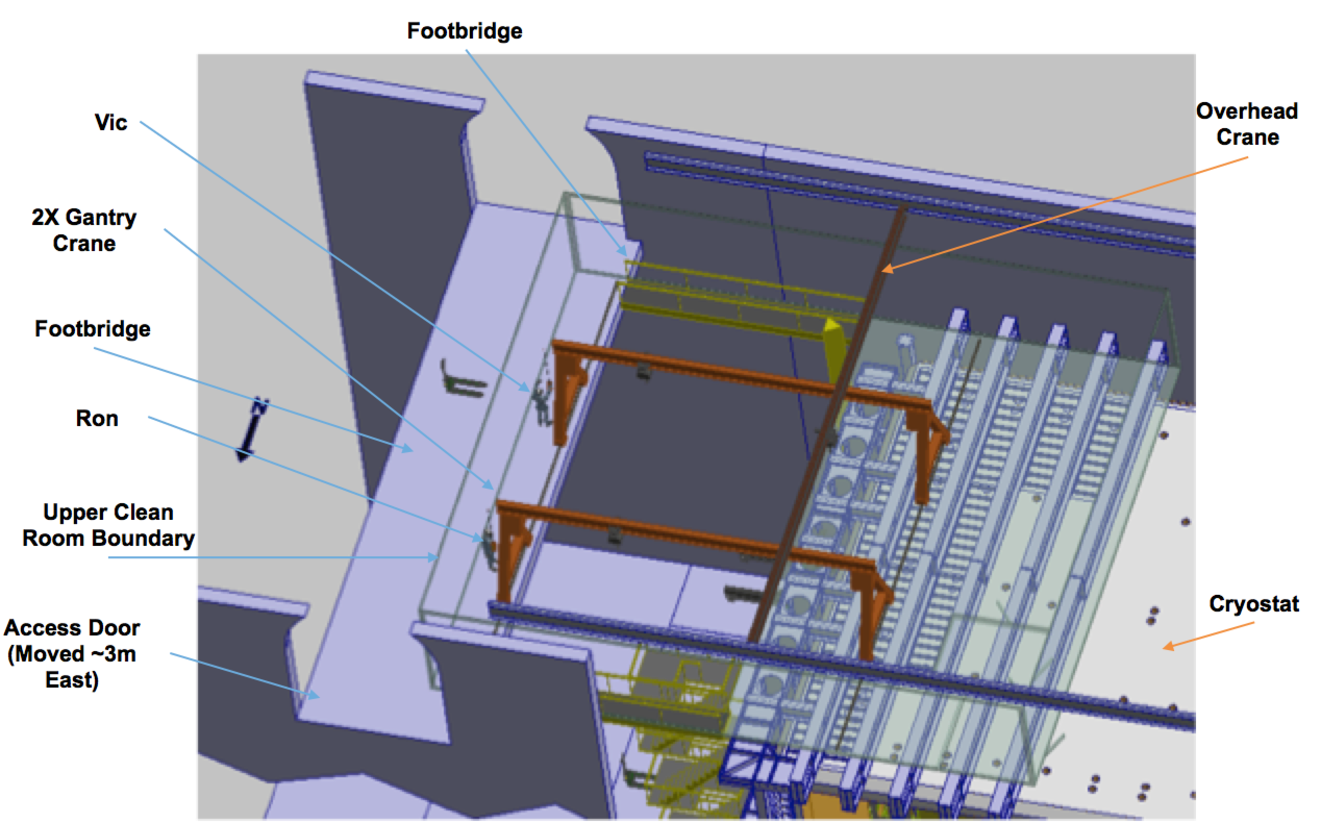
\includegraphics[width=\textwidth]{far-detector-single-phase/figures/Install-ISO-Top.pdf}
\end{minipage}
\begin{minipage}[c]{0.49\textwidth}
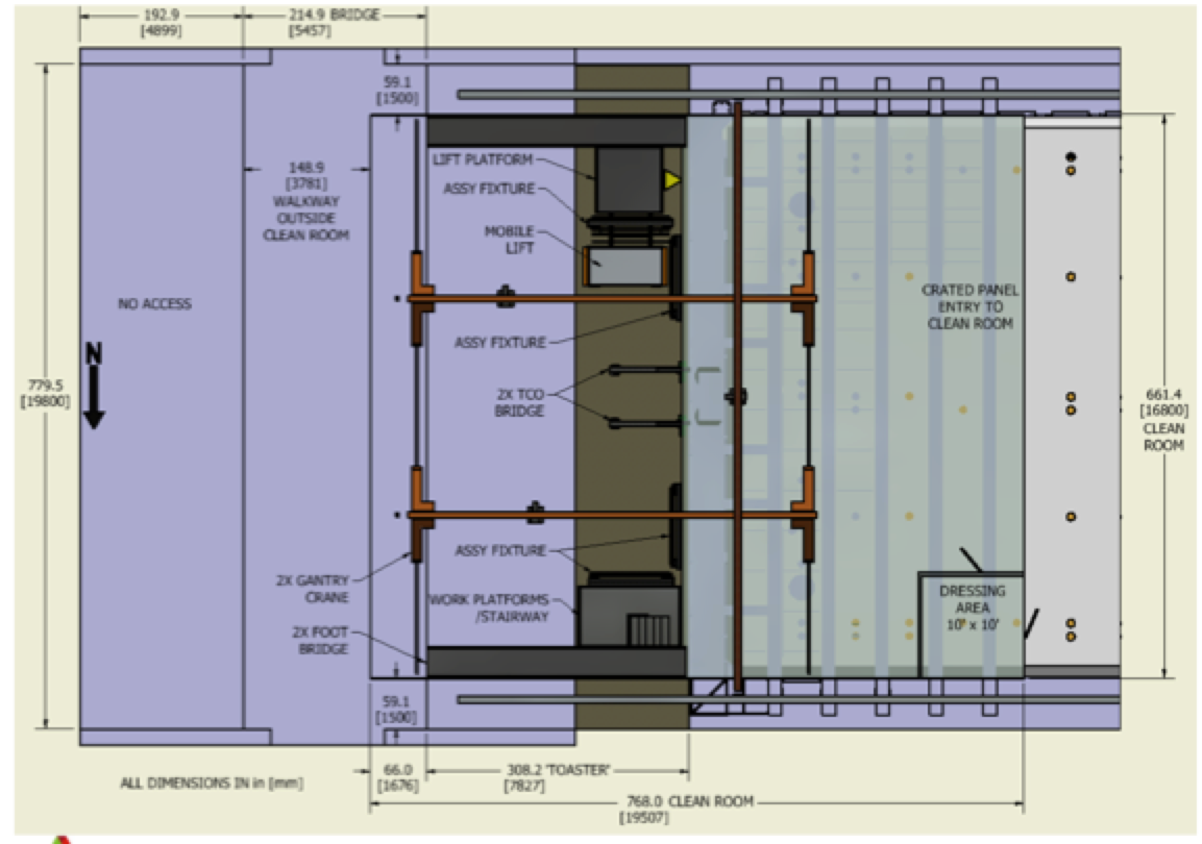
\includegraphics[width=\textwidth]{far-detector-single-phase/figures/Install-TopView.pdf}
\end{minipage}
%
\vspace{5mm}
\hrule
\vspace{5mm}
%
\begin{minipage}[c]{0.32\textwidth}
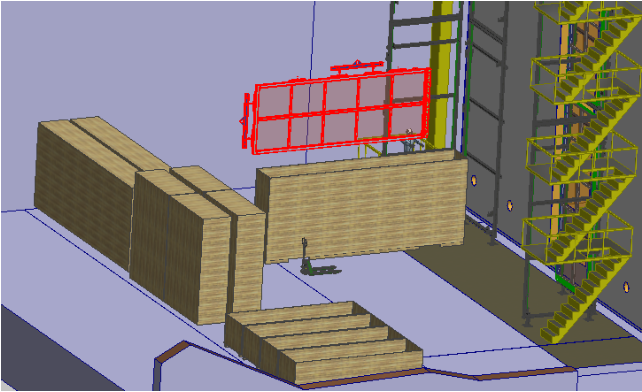
\includegraphics[width=\textwidth]{far-detector-single-phase/figures/APA-1.pdf}
\end{minipage}
\begin{minipage}[c]{0.32\textwidth}
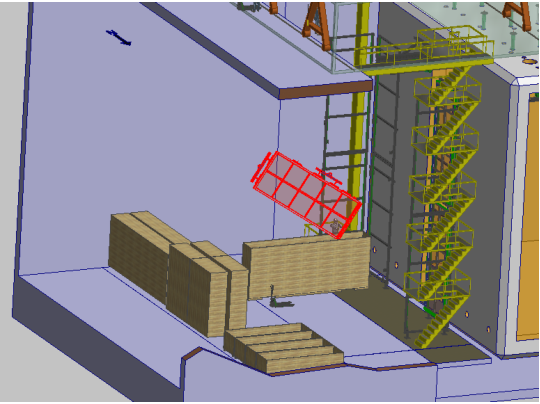
\includegraphics[width=\textwidth]{far-detector-single-phase/figures/APA-2.pdf}
\end{minipage}
\begin{minipage}[c]{0.32\textwidth}
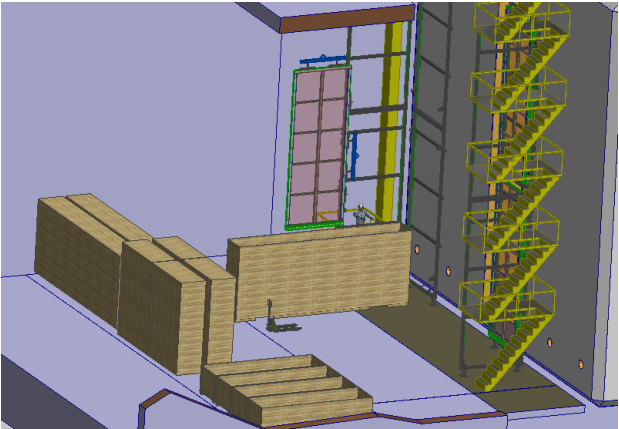
\includegraphics[width=\textwidth]{far-detector-single-phase/figures/APA-3.pdf}
\end{minipage}
%
\vspace{5mm}
\hrule
\vspace{5mm}
%
\begin{minipage}[c]{0.32\textwidth}
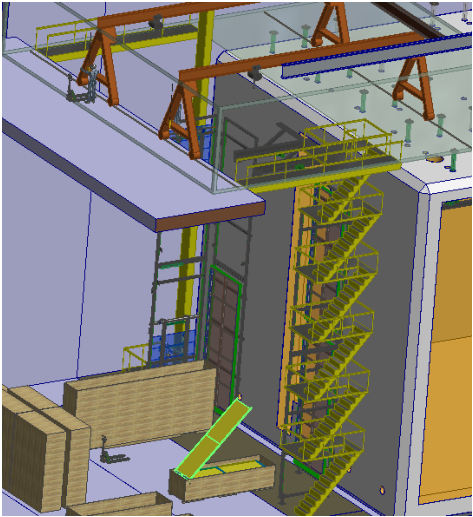
\includegraphics[width=\textwidth]{far-detector-single-phase/figures/CPA-1.pdf}
\end{minipage}
\begin{minipage}[c]{0.32\textwidth}
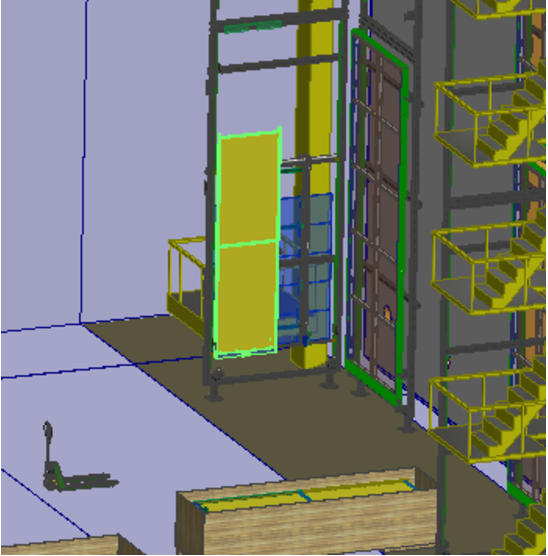
\includegraphics[width=\textwidth]{far-detector-single-phase/figures/CPA-2.pdf}
\end{minipage}
\begin{minipage}[c]{0.32\textwidth}
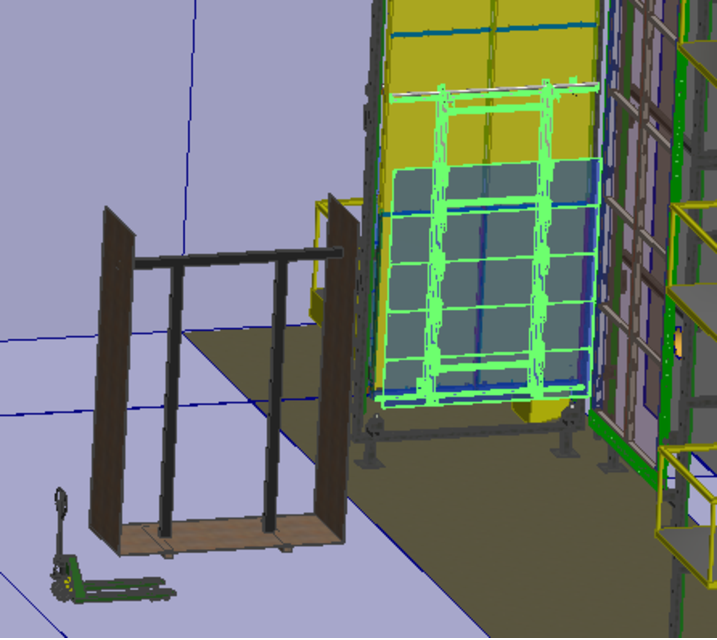
\includegraphics[width=\textwidth]{far-detector-single-phase/figures/CPA-3.pdf}
\end{minipage}

\caption{Single-Phase Detector Installation sequence}
\label{Install-Seq}
\end{center}
\end{figure}

The current installation plan is described. \dword{dune} will take
ownership of the different underground areas at different times. The
surface data room and the underground room in the CUC are available
significantly before the collaboration has access to the cryostats and
the optical fibers between the surface and underground will be in
place even earlier. This will allow a DAQ prototype to be developed
and tested early. The installation of the DAQ hardware can also be
finished before the start of detector installation if desired so the
DAQ will not be on critical path.  When the collaboration receives
access to Cryostat~\#1 the steel work for Cryostat~\#2 will be
finished and the work on installing the membrane will have
started. Excavation will be complete.  For planning purposes it is
assumed that the first detector will be \dword{sp} and the second
\dword{dp}. The first step in the \dword{sp} installation is to
install the cryo-piping and the \dword{dss}. As the cryo-piping will
require welding and grinding it is a dirty process and must be
complete before the area can be used as a cleanroom. When this is
complete the cryostat can be cleaned and the false floor
re-installed. The clean infrastructure needed to install the detector
including the cleanroom, work platforms, scaffolding, and the
fixturing to hold the detector elements during assembly and all the
lifts need to be set up. Once the infrastructure is in place and the
area clean the installation of the main elements can start. The
general layout of the installation area showing the necessary space
and equipment is shown in the top panels in Figure~\ref{Install-Seq}.

The \dword{sp} detector is installed by first installing the west endwall or
endwall~\#1 (see Fig.~\ref{fig:endwall}).
\begin{figure}[htbp]
\begin{center}
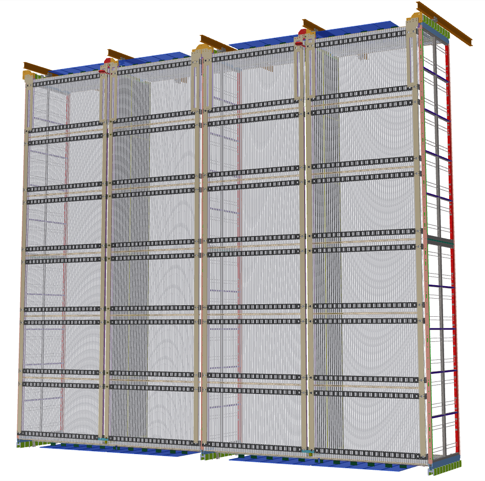
\includegraphics[width=0.4\textwidth]{endwall.png}
\caption{End view of \dword{sp} detector with endwall field cage in
  place, along with one row of \dword{apa} and \dword{cpa}.}
\label{fig:endwall}
\end{center}
\end{figure}
The \dwords{apa} and \dwords{cpa} with top/bottom FC panels are
installed next. The plan is to install \num{6} \dwords{apa} and \num{4}
\dwords{cpa} per week which is enough to complete one of the \num{25}
rows every week. Additional time is built into the schedule to take
into account that the installation will be slower at the beginning and
some re-work may be needed. By building west-to-east complete rows can
be finished and tested before moving to the next row. This reduces the
risk that after final FC deployment and cabling that a fault is found
which would require dismantling part of the detector. Some of the steps
needed to install the \dword{apa} and \dword{cpa} modules outside the
cryostat are also shown in Figure~\ref{Install-Seq}.  The middle three
panels show how the \dword{apa} needs to be handled in order to rotate
it and mount it to the assembly frame. After two \dword{apa} are
mounted on top of each other the cabling for the lower \dwords{apa}
cold electronics and photon detector cables can be installed. The
lower three panels show how the \SI{2}{m} \dword{cpa} sub-panels are
removed form the transport crates and assembled on holding frame. Once
the \dword{cpa} module is assembled the Field Cage units can them be
mounted. Finally once the \dword{apa} and \dword{cpa} are installed
the endWall~\#2 can be installed. A high level summary of the schedule
is shown in Figure~\ref{Install-Schedule}.
\begin{figure}[htbp]
\begin{center}
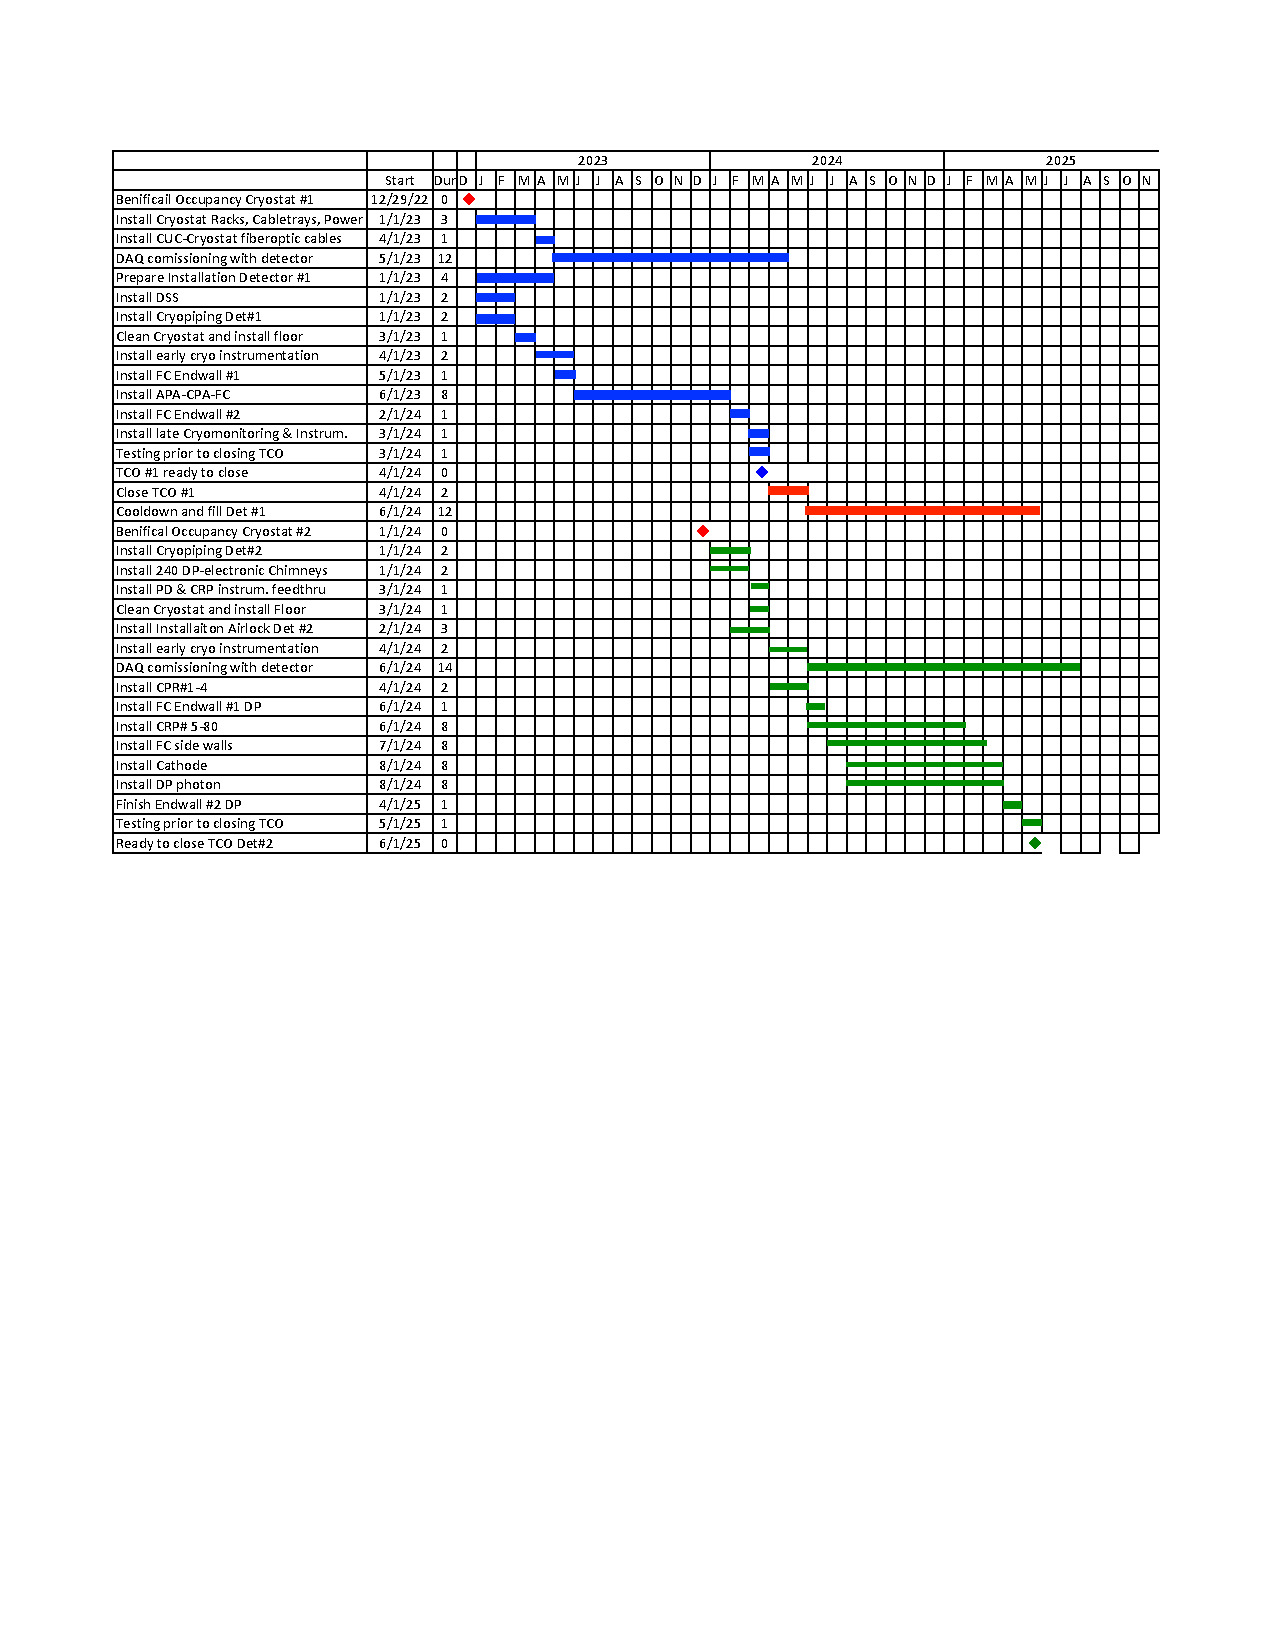
\includegraphics[width=\textwidth]{far-detector-single-phase/figures/TP-Schedule-Feb2018.pdf}
\caption{High level installation schedule}
\label{Install-Schedule}
\end{center}
\end{figure}



As is seen in the installation schedule the second cryostat becomes
available four months before the first detector installation is
complete. In this period installation work for both detectors will
proceed in parallel. Like the \dword{sp} detector the first step is
the installation of the cryo-piping followed by a thorough cleaning
and installation of the false floor. While the cryo-piping is being
installed the \dword{dp} chimneys for the electronics along with the
DPPD and CRP instrumentation feedthrus can also be installed. The
chimneys are installed into the roof of the cryostat so this work is
performed well away from the final installation work on the first
detector so there should be no conflicts. Once the first detector is
installed work on setting up the second detector installation
infrastructure can begin. This work includes moving the cranes and
work platforms along with moving the walls of the cleanroom so the
second cryostat is clean. The air filtration to the cryostat will also
be moved to the second cryostat.  Much of the work for the \dword{dp}
installation will be performed inside the cryostat so in principal a
smaller cleanroom area outside the cryostat is needed. However for
planning purposes it will not be completely sure what type detector
will be installed in the second cryostat until fairly late so the \dword{uit}
will plan to provide a sufficiently large area outside the cryostat to
accommodate either detector technology.  The\dword{dp} detector itself
would require a much smaller cleanroom which could be installed just
outside the \dword{tco}. The installation process inside the detector will
proceed East to West. At the start of the TPC installation the first
\num{4} CRP will be installed which comprises the first row of
CRP. The left panel in Figure~\ref{fig:CRP-Install} shows two CRPs
being installed near the roof of the cryostat and the right panel
shows one of the CRP in a transport box being moved into the cryostat.
Once the first CRP row is installed and tested then the first field
cage endwall can be installed. In general rows of CRP will be
installed and then behind them rows of field cage modules are
installed followed by the cathode installation at the bottom of the
detector and the photon detector PMTs under the cathode plane. Finally
at the end of the installation the second field cage endwall is
installed and a final testing period for the full detector is
foreseen. The \dword{dp} installation sequence is shown in green in
Figure~\ref{Install-Schedule}.
\begin{figure}[htbp]
\begin{center}
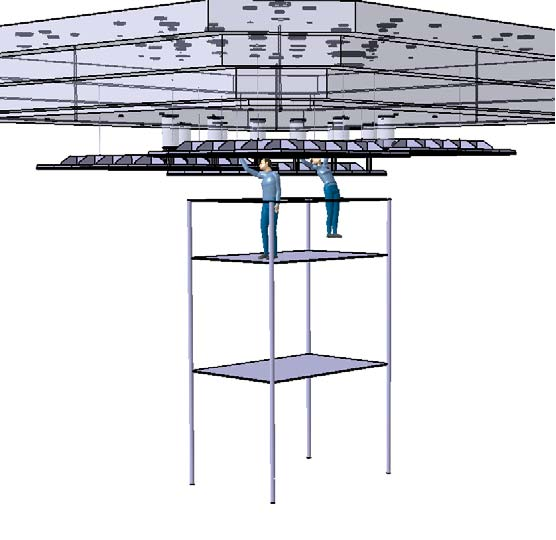
\includegraphics[width=0.4\textwidth]{far-detector-single-phase/figures/CRP-install.pdf}
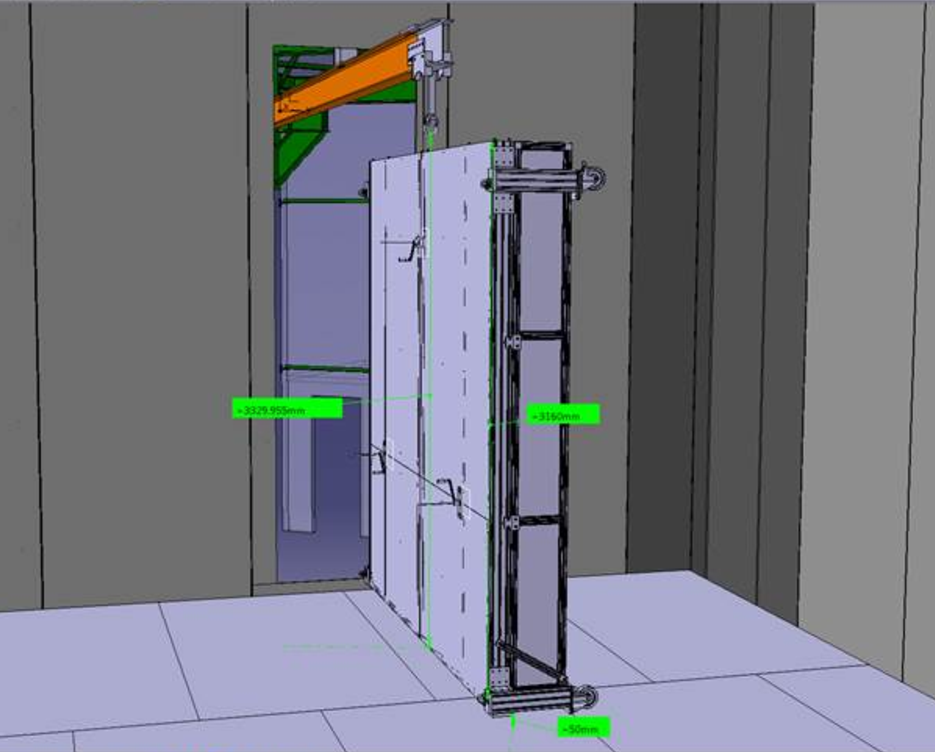
\includegraphics[width=0.4\textwidth]{far-detector-single-phase/figures/CRP-into-cryostat.pdf}
\caption{Left: Image of the \dword{dp} \dwords{crp} being installed in
  the detector, showning the connection from the \dword{crp} to the
  electronics readout chimney. Right: Image of the \dword{crp} being
  inserted into the cryostat using a transport beam.  The DP field
  cage modules will be inserted in a similar fashion.}
\label{fig:CRP-Install}
\end{center}
\end{figure}



Prior to the TDR mutually agreed upon installation plans will need to
be approved. These will set the schedule for the installation and will
determine the planning for staffing and budget. Having good estimates
for the time needed and having enough experience to ensure the
interfaces are understood and the procedures are complete is important
for accurate planning. The experience at \dword{protodune} will be
very important as the \dword{protodune} installation establishes the
procedures for handling all the detector elements and in many cases
gives accurate estimates for the time needed. However in the case of
the \dword{sp} detector many of these procedures need to revised or
newly developed as the \dword{dune} detector will be twice as high as
\dword{protodune} so two \dwords{apa} need to be assembled together
and then a totally different cabling scheme is needed. Testing the
cabling will need to be complete prior to the TDR as this is needed to
ensure the design is viable. The \dword{dp} will also need to develop
installation procedures as the \dword{dune} \dword{dp} detector
will have a significantly different field cage and cathode plane. 

The installation by definition is on the critical path making it vital
that the work be performed efficiently and in a manner that has low
risk. In order to achieve this a prototype of the installation
equipment for the \dword{dune} \dword{sp} will be constructed at Ash
River and the installation process tested with dummy detector
elements. It is expected that the setup will be available at the time
of the TDR, but any lessons learned will need to be implemented and
tested after this. In the period just prior to the start of
installation the Ash River setup will be used as a training ground for
the \dword{uit}.

%The \dword{uit} is responsible for delivering the common infrastructure
%the detector will need to operate. This infrastructure is typically
%equipment that is used by many groups. This may include: the
%electronics racks with power and cooling, cable trays, the cryostat
%crossing tubes and flanges, rigging equipment, some tools, the ground
%monitoring and isolation transformers, necessary diagnostics equipment
%(including oscilloscopes, a network analyzers and leak detector), a
%small machine shop, storage with some critical supplies, and some PPE.


%\subsection{Detector Support}

The Detector Support System (DSS) provides the structural support for
the single-phase detector inside the cryostat.  It also provides the
necessary infrastructure to move the detector elements into location
during assembly. As the DSS is a new design and is quite different
from the ProtoDUNE DSS it is described in some detail in this
section. The detector elements supported by the DSS include the field
cage endwalls, the \dwords{apa}, and the \dwords{cpa} with top and
bottom field cage panels.  The DSS is supported by the cryostat outer
steel structure through a series of feedthrus which cross through the
cryostat insulation and are anchored with flanges on the cryostat
roof. Inside the cryostat a series of stainless steel I-beams are
connected to the feedthrus and used to support the detector. The DSS
defines the location of the detector inside the cryostat and it also
defines how the detector elements move/contract as the detector is
brought to \dword{lar} temperature. The design of the DSS encompasses
the overall structural design of the detector as only after the
elements are mounted to the DSS and are connected together do they
make a unified mechanical structure. The requirements of the DSS are
as follows:
\begin{itemize}
 \setlength\itemsep{1mm}
\setlength{\parsep}{1mm}
\setlength{\itemsep}{-5mm}
% \small
\item Support the weight of the detector.
\item Accommodate the cryosat roof movement during cryostat filling, testing, and operation.
\item Accommodate variation in the feedthrough locations and
  variation in the flange angles due to installation tolerances and
  loading on the warm structure.
\item Accommodate shrinkage of the detector and DSS from ambient
  temperature to \dword{lar} temperature.
\item Define the position of the detector components relative to each other. 
\item The DSS is electrically connected to the cryostat ground and electrically isolated from the detector.
\item The DSS support penetrations must be purged with GAr to prevent contaminants from diffusing back into the liquid
\item The instrumentation cabling must not interfere with the DSS.
\item The DSS components must be able to be installed through the TCO
\item The DSS is to designed to meet AISC-360 and appropriate codes required by SURF
\item The DSS will be designed to meet seismic requirements 1 mile underground at SURF
\item All materials must be compatible for operation in ultrapure \dword{lar}
\item The DSS beams will be completely submerged in \dword{lar}
\item The DSS will ensure that detector components shall not be less than \SI{400}{mm} from the membrane flat surface
\item The DSS supports shall not interfere with the cryostat I-beam structures
\item The DSS shall be designed such that it supports the detector so that the lower ground plane is above the cryogenic piping and the top of the DSS beams are submerged in \dword{lar} while leaving a 4\% ullage at the top of the cryostat.
\item The DSS shall have infrastructure necessary to move the \dword{apa} and \dword{cpa}-FC assemblies from outside the cryostat through the TCO and to the correct position.
\end{itemize}

Figure~\ref{DSS} (left) shows the DSS structure; there are five rows
of supports for the alternating rows
of \dword{apa}-\dword{cpa}-\dword{apa}-\dword{cpa}-\dword{apa}.  The
DSS is connected to the warm structure at a flange that is mounted on
the outside of the cryostat.  Figure~\ref{DSS} (right) shows the
layout of these structural feedthroughs.  The DSS consists of pairs of
feedthroughs that support \SI{6.4}{m}-long S8x18.4 stainless steel I-beam
sections. The proposed design of the DSS has \num{10} I-beam segments per
row for a total of \num{50} I-beam segments. Each I-beam is suspended on
both ends by rods from feedthroughs that penetrate the roof.  In the
cold condition each beam will shrink which will cause gaps to form
between \dwords{apa} that are adjacent but supported on separate
beams.  \dwords{apa} that are supported on the same beam will not have
gaps develop because both the beam and \dwords{apa} are stainless
steel so they will shrink together.  Each beam is supported by a
nearly \SI{2}{m} long rod that allows the beam support to move as the beam
contracts.
%\fixme{too much detail}
%The feedthrough consists of a flange and $8 ^{''}$ OD structural tube
%welded to it that extends through the cryostat insulation.  There is a
%nominal \SI{10}{mm} gap between the OD of the tube and the ID of the
%clearance tube in the cryostat.  The purpose of the $8 ^{''}$ tube is
%to provide lateral support to the I-beams during installation.
%Running down the center of the feedthrough is a $1^{"}$ diameter rod that
%is supported at a swivel washer at the flange and then supports the
%I-beam at a clevis.  The gas seal is obtained by Conflat Flange and a
%bellows that seals around the swivel washer.  The lateral position of
%the rod can be adjusted to adjust the height of the DSS I-beams.
\begin{figure}[htbp]
\begin{center}
\begin{minipage}[c]{0.49\textwidth}
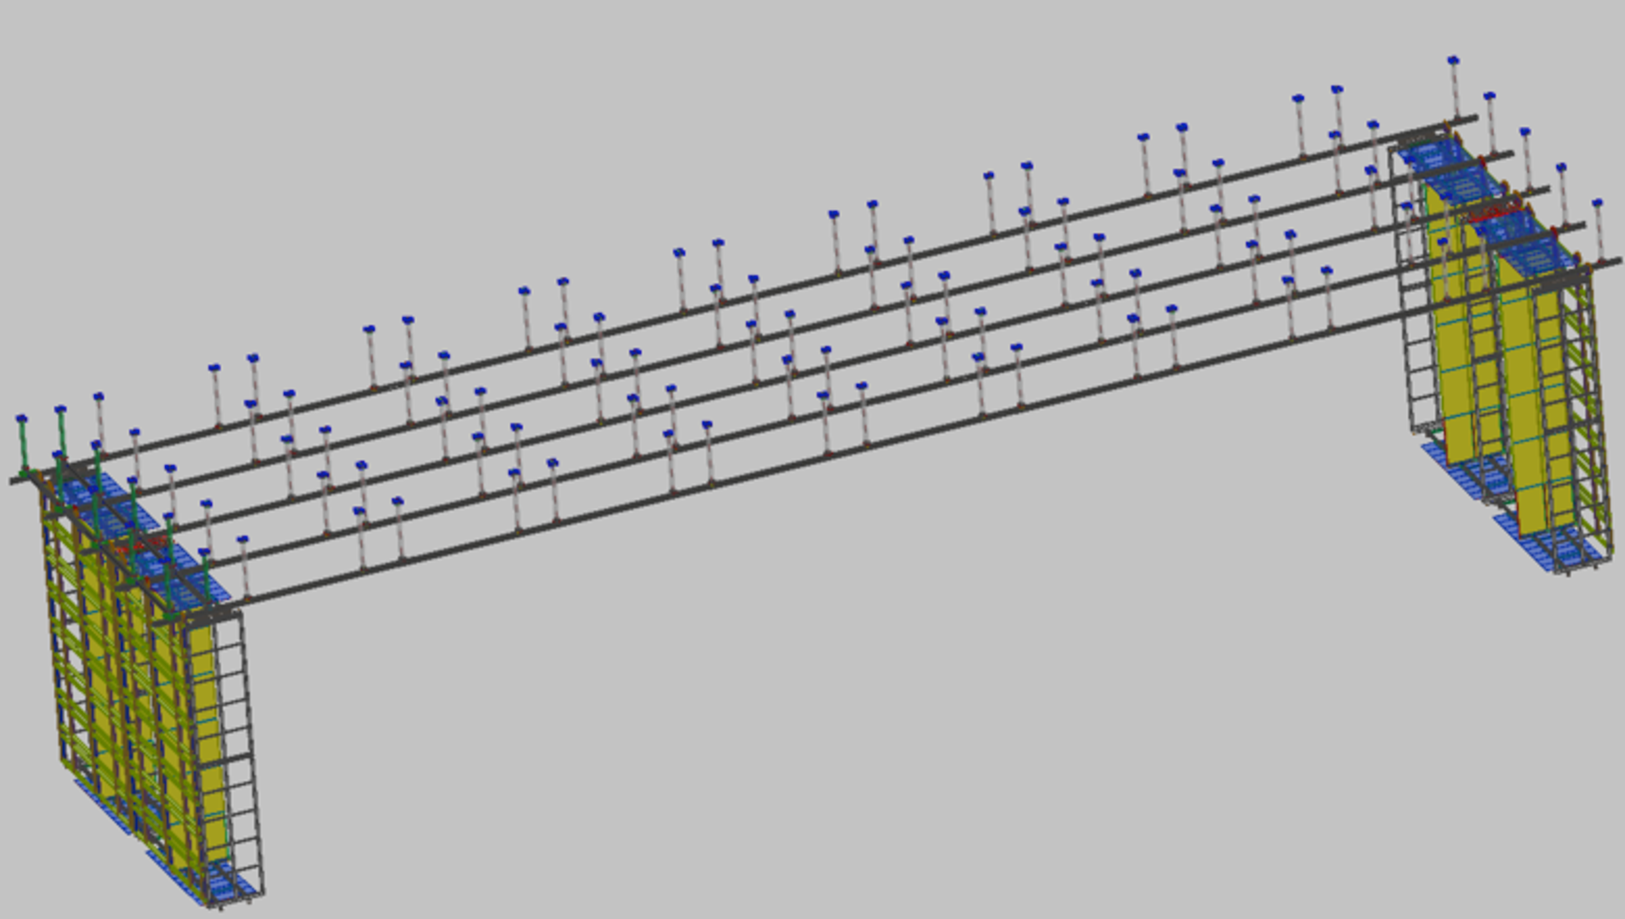
\includegraphics[width=\textwidth]{far-detector-single-phase/figures/DSS-1.pdf}
\end{minipage}
\begin{minipage}[c]{0.49\textwidth}
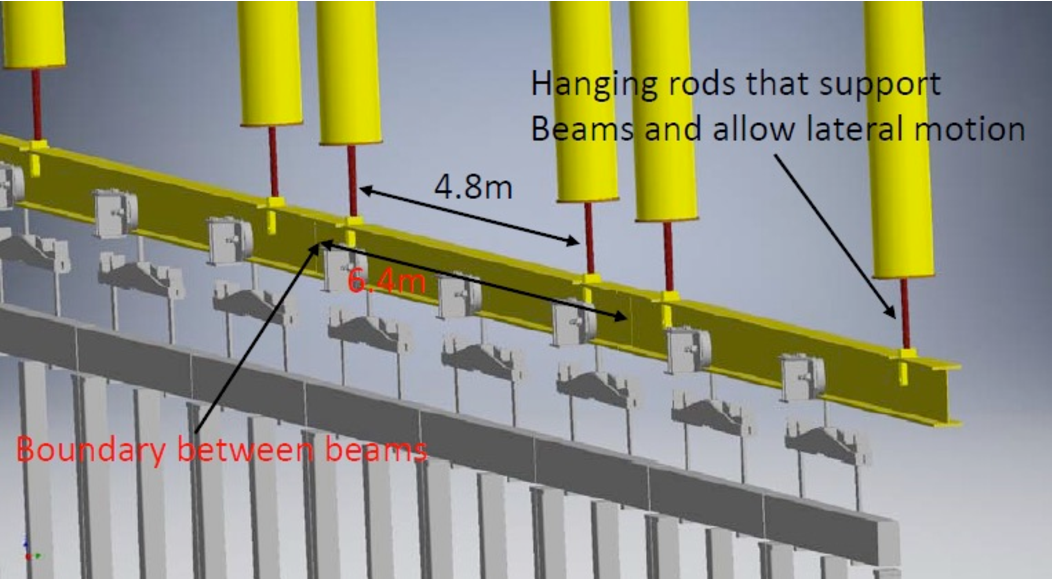
\includegraphics[width=\textwidth]{far-detector-single-phase/figures/DSS-2.pdf}
\end{minipage}
\caption{3-D model of the Detector Support System showing the entire structure on the left along with one row of \dword{apa} and \dword{cpa}/FC at each end. The right panel is a zoomed image showing the connections between the vertical supports and the horizontal I-beams.}
\label{DSS}
\end{center}
\end{figure}


Detector components will be installed using a shuttle beam system
illustrated in Fig.~\ref{shuttle}.  The last two columns of
feedthroughs (eastern most) will support temporary beams that run
north-south, perpendicular to the main DSS beams.  A shuttle beam
%shown in orange
will have trolleys mounted to it and will transverse
north-south until aligned with the required row of DSS beam.  The last
\dword{apa} or \dword{cpa} in a row is supported by the shuttle beam which is bolted
directly to the feedthroughs once it is in place.  As the last \dword{cpa} or
\dword{apa} in each row is installed the north-south beams are removed.

There will be a mechanical interlock system that prevents trolleys
from passing the end of the shuttle beam unless it is aligned with a
corresponding DSS beam.  The shuttle beam and each detector will be
moved using a motorized trolley.  A commercially available motorized
trolley will be modified as needed to meet the needs of the
installation.
\begin{figure}[htbp]
\begin{center}
\begin{minipage}[c]{0.49\textwidth}
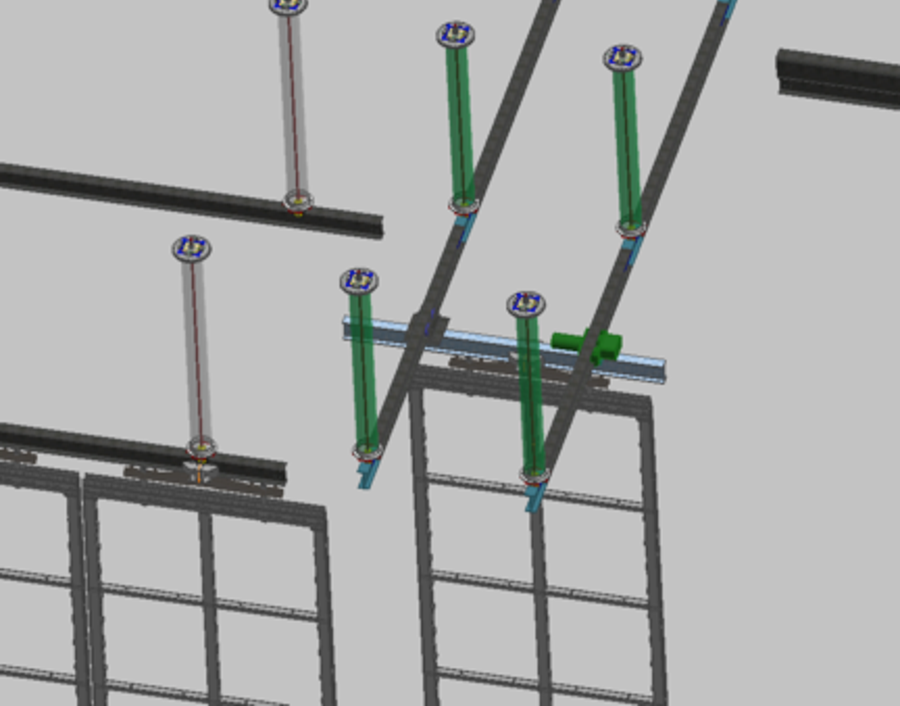
\includegraphics[width=\textwidth]{far-detector-single-phase/figures/Shuttle-1.pdf}
\end{minipage}
\begin{minipage}[c]{0.42\textwidth}
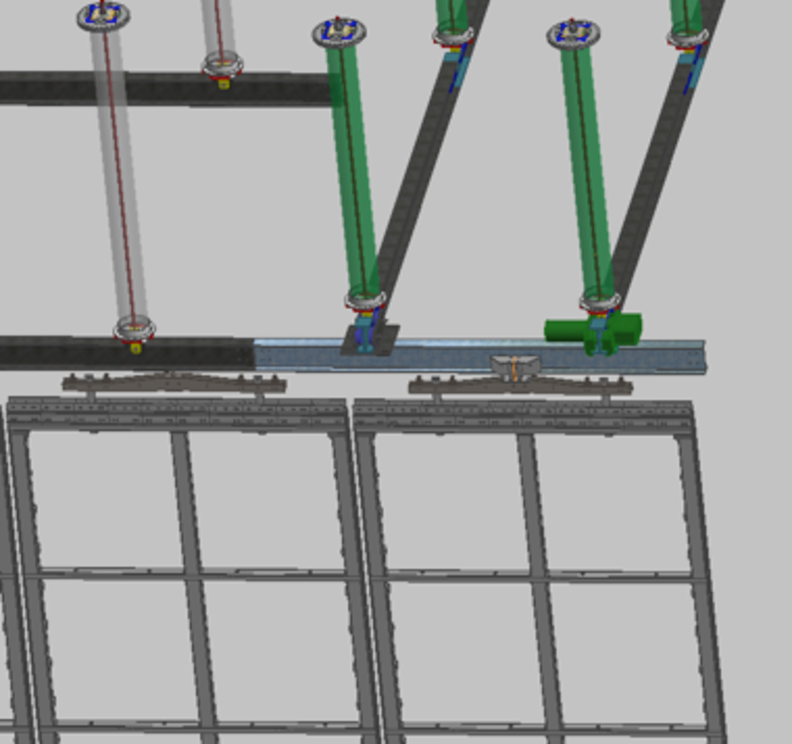
\includegraphics[width=\textwidth]{far-detector-single-phase/figures/shuttle-2.pdf}
\end{minipage}
\caption{3-D models of the shuttle beam end of the DSS. The figures show how an \dword{apa}
is translated into position using he North-South beams until it lines up with the correct
row of I-beams.}
\label{shuttle}
\end{center}
\end{figure}

The DSS installation begins with the placement and alignment of all
the feedthroughs onto the flanges that are mounted to the warm vessel.
There are \num{25} feedthroughs per row and five rows for a total of \num{125}
feedthroughs.  A fixture with a tooling ball will be attached to the
clevis of each feedthrough.  The $XY$ position in the horizontal plane
and the vertical $Z$ position of this tooling ball will be defined.  A
survey will be performed to determine the location of each tooling
ball center and $XY$ and $Z$ adjustments will be made to get the tooling
ball centers to within $\pm$\SI{3}{mm}.  The \SI{6.4}{m} long I-beams will then be
raised and pinned to the clevis.  Each beam weights roughly 350~lbs.
A lifting tripod will be placed over each of the feedthroughs
supporting a beam and a $1/4 ^{''}$ cable will be fed through the top
flange of the feedthrough down the \SI{14}{m} to the cryostat floor where it
will be attached to the I-beam.  The winches on each tripod will raise
the beam in unison in order to get it to the correct height to be
pinned to the feedthrough clevis.  Once the beams are mounted a final
survey of the beams will occur to ensure they are located and aligned
to each other properly.

A mock up of the shuttle system will be constructed to test the
mechanical interlock and drive systems for the shuttle beam
for each detector.  Tests will be conducted to evaluate the level of
misalignment between beams that can be tolerated and the amount of
positional control that can be achieved with the motorized trolley. It
is expected this will be finished prior to the TDR. At the time of the
TDR a larger prototype installation at Ash River will be under
construction. This prototype will use full scale elements and will be
used to develop the installation procedures and to also test the
detector installation process.


\subsection{Preparation for Operations}

After the detectors are installed in the cryostat there remains a lot
of work before the detectors can be operated. First the \dword{tco} must be
closed. This requires bringing back the cryostat manufacturer to close
the opening which was left in the cryostat originally for the detector
installation. First the missing panel with the steel beams and steel
panel are installed to complete the cryostat's outer structural
hull. Then the remaining foam blocks and membrane panels are installed
from the inside using the manholes for access. In parallel to this the
liquid argon pumps are installed at the ends of the cryostat and final
connections are made to the recirculation plant. Once the pumps are
installed, the cryostat is closed and everything is leak tested the
cryogenic plant can be brought into operation. First the air inside
the cryostat is purged by injecting pure argon gas at the bottom of
the detector at a rate such that the detector is filled uniformly but
faster than the diffusion rate. This produces a column of argon that
rises through the detector and sweeps out the air. This process is
referred to as the piston purge. When the piston purge is complete the
cooldown of the detector can begin. Misting nozzles inject a
liquid-gas mix into the cryostat which cools the detector at a
controlled rate. Once the detector is cold the filling process can
begin. Gaseous argon is brought from the surface down the shaft and is
re-condensed underground. The liquid argon then flows through filters
to remove any H$_2$O or O$_2$ and flows into the cryostat. Given the
very large volume of the cryostats and the limited cooling power for
re-condensing the liquid it is expected to take 12 months to fill the
first detector and 14 months to fill the second. During this time the
detector readout electronics will be on so the status of the detector
can be monitored. Once the detector is full the drift high voltage can
be carefully ramped up and data taking can begin.




